\documentclass[11pt, a4paper, twoside, titlepage, usenames,dvipsnames]{report}
\usepackage[page, title, titletoc]{appendix}
\usepackage[a4paper, total={6in, 8in}]{geometry}
\usepackage[section]{placeins}
\usepackage[utf8]{inputenc}
\usepackage{amsfonts}
\usepackage{amsmath}
\usepackage{physics}
\usepackage{adjustbox}
\usepackage{amssymb}

\let\oldemptyset\emptyset
\let\emptyset\varnothing

\setlength{\parindent}{24pt}
\newtheorem{definition}{Definition}[chapter]
\newtheorem{lemma}{Lemma}[chapter]
\newtheorem{theorem}{Theorem}[chapter]

% Set graphics folder
\usepackage{float}
\usepackage{graphicx}
\usepackage[format=plain, font=it]{caption}
\usepackage[format=plain, font=it]{subcaption}
\graphicspath{{"../../../OneDrive - Delft University of Technology/MEP - thesis Mark/Figures/ch_toric_code/"}}

% Set algorithm2e package settings
\usepackage[linesnumbered, vlined]{algorithm2e}
\SetStartEndCondition{ }{}{}
\SetKwProg{Fn}{def}{\string:}{}
\SetKw{KwTo}{in}
\SetKwFor{For}{for}{\string:}{}
\SetKwIF{If}{ElseIf}{Else}{if}{ then}{elif}{else:}{}
\SetKwFor{While}{while}{ do}{}
\SetAlgoNoEnd\DontPrintSemicolon

% Set algorithm title custom box
\usepackage[most]{tcolorbox}
\tcbset{algotitle/.style={title={ \strut Algorithm~\thetcbcounter\ifstrempty{#1}{\ignorespaces}{:~#1}}}}
\newtcolorbox[auto counter]{algo}[1][]{
    colback=white, colframe=black, boxrule=0.5pt,
    titlerule=0pt, sharp corners, colbacktitle=white,enhanced,
    attach boxed title to top center={yshift=-10pt},
    boxed title style={boxrule=-1pt},
    fonttitle=\bfseries, coltitle=black, algotitle={}, #1}

\usepackage{xcolor}
\usepackage{listings}
\usepackage{xparse}
\usepackage{todonotes}


\NewDocumentCommand{\codeword}{v}{\texttt{\textcolor{MidnightBlue}{#1}}}
\NewDocumentCommand{\codefunc}{v}{\texttt{\textcolor{OliveGreen}{#1}}}
\newcommand{\m}[1]{\mathcal{#1}}
\newcommand{\nset}{\mathcal{N}}
\newcommand{\vset}{\mathcal{V}}
\newcommand{\pre}[1]{ {}^{#1} }

\lstset{language=C,keywordstyle={\bfseries \color{blue}}}
% Set quantikz settings
\usepackage{tikz}
\usetikzlibrary{quantikz,shapes,calc}
\def\checkmark{\tikz\fill[scale=0.4](0,.35) -- (.25,0) -- (1,.7) -- (.25,.15) -- cycle;}
\SetAlFnt{\footnotesize}
\tikzset{bellstar/.style ={draw, star,star points = 8, star point height = 1em, star point ratio = 1.8, minimum size = 1em, inner sep = 0pt}}
\tikzset{selection/.style={draw, signal, signal to =south, minimum size = 1em, inner sep = 0pt}}
\tikzset{sel/.style={label position = below, yshift = 0.5cm}}


\title{mep-thesis}
\author{Shui Hu}
\date{April 2019}


\begin{document}

\begin{titlepage}
	\newcommand{\HRule}{\rule{\linewidth}{0.3mm}}
	\center

	\textsc{\Large Delft University of Technology}\\[1.5cm]

	\textsc{\large Master's Thesis}\\[0.5cm]

    \vfill

	\HRule\\[1cm]

	{\huge\bfseries Quantum Error Correction of Patch-Loss of the Surface Code}\\[0.4cm]

	\HRule\\[1.8cm]

	\begin{minipage}{0.4\textwidth}
		\begin{flushleft}
			\large
			\textit{Author}\\
			S. \textsc{Hu}
		\end{flushleft}
	\end{minipage}
	~
	\begin{minipage}{0.4\textwidth}
		\begin{flushright}
			\large
			\textit{Supervisor}\\
			D. \textsc{Elkouss} % Supervisor's name
		\end{flushright}
	\end{minipage}


	%------------------------------------------------
	%	Date
	%------------------------------------------------

	\vfill\vfill\vfill % Position the date 3/4 down the remaining page

	{\large\today} % Date, change the \today to a set date if you want to
	\vfill % Push the date up 1/4 of the remaining page

\end{titlepage}


\tableofcontents

%\chapter{Preliminary report}

\subsection*{Introduction}

Quantum computing has the potential to transcend the information technology as we know it. Small scale quantum systems are already possible today and the goal is to scale up these quantum architectures to build practical quantum devices. One approach to do this is to by networking many simple processor cells together through quantum links, avoiding the necessity to build a single complex structure. Processor cells that are located physically close to each other are connected by "short" links and lie in a patch. Patches that are located physically far from each other can in turn be connected by "long" links, such as remote optical connections. The total state of system, which contains the stored information, is shared across these patches, such that it can be accessed in either one of these patches. \\

This is somewhat analogous to the idea of a shared database. Many online services that we use today rely on servers that host the data that we want to view, store or edit. This data is often not stored on a single server, but copied to many others, in a shared database. In case one of these servers goes offline due to file corruption or an electricity outrage, the data is not lost, and can still be accessed on another server in the cluster.\\

In our Quantum network, information cannot be copied across different processor cells due to the no cloning theorem. In stead, it is shared across cells through entanglement. A cell can also go "offline", when a qubit or multiple qubits are lost from the system due to some interaction with the environment. This process is called decoherence, also described with \emph{loss} or \emph{erasure}. Luckily, if the losses are not too much, these cells can be restored through quantum error correction (QEC) such that the quantum state or encoded information can still be extracted from the system. \\

\subsection*{Quantum errors}
Errors that can occur during Quantum computation can generally be classified as 1) noise, in which there is an error are within the computational basis, or as 2) a loss, in which the qubit is
taken out of the computational basis. Losses are both detectable and locatable, which means that a higher rate of loss ($p_{loss}$) can be tolerated than noise or computational errors ($p_{com}$). The process of finding and correcting these errors is called decoding. \\

Kitaev's surfaces codes are defined by a set of stabilizers which act on a set of physical qubits that lie on the edges of a square lattice \cite{kitaev}. The stabilizers commute, and are generated by plaquettes (group of $Z$ operators), or by stars (group of $X$ operators). Logical operates corresponds to a set of stabilizer operators along a homologically nontrivial cycle. Any homologically equivalent set of operators can be used to measure the physical qubit operator. Therefore, in the case of a qubit loss, another set of operators can be used, if there is no \emph{percolated} region of losses that span the entire lattice. \\

To decode for computational errors, one measures the stabilizer generators, which returns eigenvalue -1 on the edges of the error chains or syndromes, and can be corrected by finding a nontrivial closing chain, which either equals a stabilizer measurement that corrects the error, or a logical operator which equals a logical error. This problem is equivalent to the two dimensional random-bond Ising model (RBIM), where the shortest path needs to be found between matching pairs. The closing chain is found using the Edmonds' minimum weight perfect matching (MWPM) algorithm. This algorithm scales quadratic in time as the lattice size increases \cite{stace2009}. More recently, an almost-linear decoding approach has been described by Delfosse et al. \cite{nickerson2017}. \\

There are also multiple methods to decode for losses on the surface code. Stace et. al \cite{stace2009,stace2010} describes the method of so-called superplaquettes and superstars, in which the lost qubit is accounted for by combining neighboring stabilizers. The resulting lattice can be than decoded using the same MWPM algorithm. Delfosse et al \cite{delfosse2017} describes a linear-time maximum likelihood method to decode for losses. Here, the errors are found in a \emph{peeling} algorithm that iteratively peels branches away from a tree of possible error chains until the lost qubits remain.

\subsection*{Patch loss}
In terms of the surface code, a patch is a set of neighboring qubit cells on the lattice that lie physically close to each other. The entire lattice is built by connecting multiple patches. It is possible that cells within the same patch suffer the same decoherence, due to their physical vicinity, such that entire patches may be lost. The Quantum links that connect these patches, in turn, may suffer a larger amount of noise due to the distance it must cross. \\

These patch losses may be investigated using the decoding algorithms described above. There are two main question to be answered here. The first one involves the size of the patches. What are tolerable sizes of patches such that in the event of a patch loss, the encoded Quantum information can still be extracted from the system? The second question concerns the Quantum links between these patches. What effects does the patch model on the surface have on the tolerable noise thresholds, especially on the thresholds of the Quantum links that connect different patches?

\subsection*{Project}
This project will focus on the two problems of the patch model described in the previous section. We will use simulations to calculate for the thresholds on patch sizes and noise. Most probably, we will try to build this simulation on top of the fault-tolerance simulations by N. Nickerson \cite{naomi}, whose thesis will also be used as our foundation on quantum error correction. Furthermore, the introduction on topological codes will be provided by the lecture notes of D. Browne \cite{browne}. We we use the knowledge acquired in the courses Advanced Quantum Mechanics (AP3051G), Computational Physics (AP3082D), as well as the EDX courses The Building Blocks of a Quantum Computer (DelftX - QTM2x, QTM3x) and Quantum Cryptography (CaltechDelftX - QuCryptox), which are similar to the TU Delft courses AP3421 and CS4090. \\

The project will be done under supervision of David Elkouss, who leads the Elkouss group, which is part of the Roadmap Quantum Internet and Networked Computing at QuTech. Weekly meetings are planned for discussions and evaluations. A presentation for the group will be held after a month. Furthermore, we also expect to be working closely together with Sebiastian de Bone, who is a Phd student at the Elkouss Group.\\

\noindent
The project can be divided into 5 successive objectives:
\begin{enumerate}\label{test}
  \item Theory and prediction of model with patch-loss of the surface code.
  \item Calculation of threshold on patch sizes.
  \item Definitions of noise between patches.
  \item Combine patch-loss and noise between patches.
  \item Improve decoder.
\end{enumerate}
The preparation for the master thesis ends on April 12, 2019. From here, the first 3 months of the project, until July 2019, we expect to be working on objective 1, expanding our theoretical knowledge of the Quantum erasure code and formulating definitions of the patch model. Ideally, we will also have some simulations results for objective 2 by the end of July. We will take a short break in August, whereafter we will continue on objectives 3 and 4. Objective 5, improving the decoder, is an optional objective. The mechanism of the decoders are so complicated, that an improvement may be a project on its own. However, due to my particular interest in these decoders, I will be alert on trying to find a point of improvement if possible. The timeline of this project will look as such.
\begin{figure}[htpb]
  \centering
  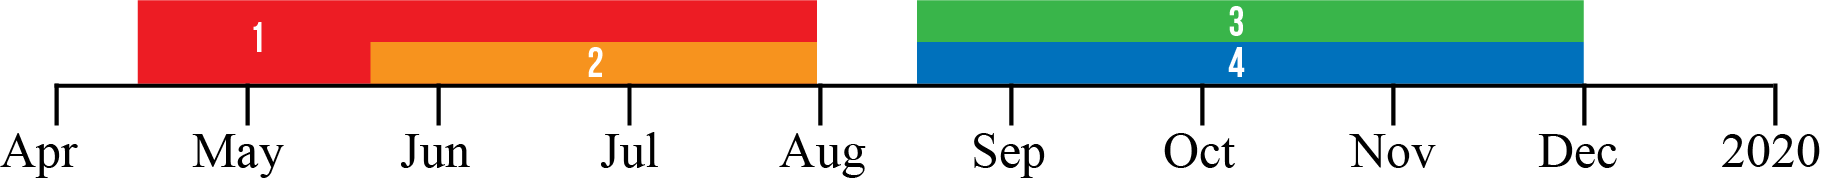
\includegraphics[width=\linewidth]{fig/Timeline.png}
\end{figure}

If the simulation of the patch sizes (2) will be so complicated such that after it cannot be completed before the end of July, we will drop objectives 3 and 4 and focus on the first two objectives. The deadline for the thesis is set to the end of November, such that a defense may be held in December.


%In the case that $p_{com} = 0$, the threshold for logical qubit recovery is $p_{loss} < 0.5$, which is equivalent to the \emph{bond percolation threshold}. In the case that $p_{loss} = 0$, computational errors can be found by measuring the stabilizer generators, which returns eigenvalue -1 on the edges of the error chains or syndromes, and can be corrected by finding a nontrivial closing chain, which either equals a stabilizer measurement that corrects the error, or a logical operator which equals a logical error. This problem is equivalent to the two dimensional random-bond Ising model (RBIM), where the shortest path needs to be found between matching pairs. The closing chain is found using the Edmonds' minimum weight perfect matching (MWPM) algorithm. In this case, the threshold is $p_{com} < 0.104$, for which a larger lattice size will decrease the chance of a logical error. These two thresholds corresponds to two end points of a boundary of correctability: $(p_{loss}, p_{comp}) = (0.5,0)$ and $(0,0.104)$.\\

%\subsubsection*{Superstabilizer decoder\cite{stace2009,stace2010}}
%To correct for losses on the surface code, new stabilizer generators are formed by connecting neighboring plaquettes or stars, which are connected to the same lost qubit, forming so-called superplaquettes and superstars respectively. These superstabilizers may share multiple qubits, and a nontrivial error chain arises of there are an odd number of (computational) errors in these shared qubits. This can be avoided by degrading the edges (shared qubits) between the superstabilizers to a single superedge whose error rates depend on the number of physical qubits shared, accounting for this degeneracy. For the sake of computation it is easier to stay on a square lattice. Take each stabilizer as a node and each shared qubit as an edge. The superstabilizer approach can be achieved by setting the weight of the edge of a lost qubit to 0, and the weight of shared edges between superstabilizers to the weight of the superedge. \\

%Using the superstabilizer approach, Edmonds' MWPM algorithm can be applied with altered edge weights. Simulations using the superstabilizers scheme with varying $p_{loss}$ show that the computational error threshold $p_{comp}^{thr}$ stay within the boundary of correctability, following the universal scaling law. At the limit of small $p_{loss}$, superstabilizer mostly consist of only 6 qubits, and increasing $p_{loss}$ only contributes to the number of superstabilizers, resulting in a linear relationship of threshold $p_{comp}^{thr}$ with $p_{loss}$.   As $p_{loss}$ increases further, larger superstabilizers containing more qubits appear, which have an increased chance of syndrome error. At $p_{loss} > 0.425$, the universal scaling law breaks down due to the size of the superstabilizers, as finite lattice effects dominate.\\

%One must also take into account that some error matchings may have a higher path degeneracy than others, indicating that the former is more likely. Therefore, the weights of the edges must additionally account for this degeneracy. However, due to this notion it possible that the algorithm may favor a matching that is not necessarily the shortest path. To balance these factors an additional factor $\tau$ is introduced that specifies the importance of path degeneracy. An optimal value for $\tau$ is found for which the computational error threshold is increased to $p_{comp}^{thr} = 0.1065$. Various implementations of Edmonds' MWPM algorithms are tested not to account for this degeneracy, and therefore a higher threshold may be possible with a computationally efficient algorithms that takes this into account.

%\subsubsection*{Maximum likelihood decoder\cite{delfosse2017}}
%Another way to look at erasure, is that the lost qubit is replaced by a maximally mixed state, which can also be interpreted as a qubit suffering a Pauli error $I,X,Y,Z$ chosen at random. Just as before, the decoding is done by measuring the plaquettes and stars, except now there is the additional knowledge of the erasure pattern, in which the errors must occur.\\

%For a set of errors $\sigma$ in the erasure pattern $\varepsilon$, either $X$ or $Z$ errors ($Y$ is a combination of the two), the algorithm is to make a spanning forest $F_{\varepsilon}$ inside of $\varepsilon$, a maximal subset of edges of $\varepsilon$ that contains no cycles. From this tree, boundary edges called leafs are iteratively stripped from $F_{\varepsilon}$. If the single connected vertex of the leave is in $\sigma$, the leaf or edge is added to the correction chain, and the other vertex is flipped in $\sigma$. What remains after the stripping $F_{\varepsilon}$ is the correction chain. On surface codes with boundaries, additional constrains are applied to the method of how the spanning forest is grown. \\

%\subsubsection*{Comparison}
%The benefit of the maximum likelihood decoder is that it scales linear with the size of the surface code. The spanning forest can be grown in linear-time, and the stripping process also only passes each leaf once, ensuring linear complexity. The superstabilizer decoder applies Edmonds' algorithm, which scales quadratic in time, but does however solve for erasure and computation errors simultaneously, whereas the maximum likelihood decoder only solves for erasure errors. Therefore, the optimal decoder probably depends on the size of the system.


\chapter{Introduction}


Quantum computing has the potential to transcend the information technology as we know it. Small scale quantum systems are already possible today and the goal is to scale up these quantum architectures to build practical quantum devices. One approach to do this is to by networking many simple processor cells together through quantum links, avoiding the necessity to build a single complex structure. Processor cells that are located physically close to each other are connected by ``short'' links and lie in a patch. Patches that are located physically far from each other can in turn be connected by ``long'' links, such as remote optical connections. The total state of system, which contains the stored information, is shared across these patches, such that it can be accessed in either one of these patches. \\

This is somewhat analogous to the idea of a shared database. Many online services that we use today rely on servers that host the data that we want to view, store or edit. This data is often not stored on a single server, but copied to many others, in a shared database. In case one of these servers goes offline due to file corruption or an electricity outrage, the data is not lost, and can still be accessed on another server in the cluster.\\

In our Quantum network, information cannot be copied across different processor cells due to the no cloning theorem. In stead, it is shared across cells through entanglement. A cell can also go ``offline", when a qubit or multiple qubits are lost from the system due to some interaction with the environment. This process is called decoherence, also described with \emph{loss} or \emph{erasure}. Luckily, if the losses are not too much, these cells can be restored through quantum error correction (QEC) such that the quantum state or encoded information can still be extracted from the system. \\

\subsection{Quantum errors}
Errors that can occur during Quantum computation can generally be classified as 1) noise, in which there is an error are within the computational basis, or as 2) a loss, in which the qubit is
taken out of the computational basis. Losses are both detectable and locatable, which means that a higher rate of loss ($p_{loss}$) can be tolerated than noise or computational errors ($p_{com}$). The process of finding and correcting these errors is called decoding. \\

Kitaev's surfaces codes are defined by a set of stabilizers which act on a set of physical qubits that lie on the edges of a square lattice \cite{dennis2002topological}. The stabilizers commute, and are generated by plaquettes (group of $Z$ operators), or by stars (group of $X$ operators). Logical operates corresponds to a set of stabilizer operators along a homologically nontrivial cycle. Any homologically equivalent set of operators can be used to measure the physical qubit operator. Therefore, in the case of a qubit loss, another set of operators can be used, if there is no \emph{percolated} region of losses that span the entire lattice. \\

To decode for computational errors, one measures the stabilizer generators, which returns eigenvalue -1 on the edges of the error chains or syndromes, and can be corrected by finding a nontrivial closing chain, which either equals a stabilizer measurement that corrects the error, or a logical operator which equals a logical error. This problem is equivalent to the two dimensional random-bond Ising model (RBIM), where the shortest path needs to be found between matching pairs. The closing chain is found using the Edmonds' minimum weight perfect matching (MWPM) algorithm. This algorithm scales quadratic in time as the lattice size increases \cite{stace2009thresholds}. More recently, an almost-linear decoding approach has been described by Delfosse et al. \cite{delfosse2017linear}. \\

There are also multiple methods to decode for losses on the surface code. Stace et. al \cite{stace2009thresholds,stace2010error} describes the method of so-called superplaquettes and superstars, in which the lost qubit is accounted for by combining neighboring stabilizers. The resulting lattice can be than decoded using the same MWPM algorithm. Delfosse et al \cite{delfosse2017linear} describes a linear-time maximum likelihood method to decode for losses. Here, the errors are found in a \emph{peeling} algorithm that iteratively peels branches away from a tree of possible error chains until the lost qubits remain.

The Union-Find decoder is preferred over other types of decoders because it is \emph{simple}. Even though it may not seem so due to the length of its chapter, the concept of the Union-Find decoder is much more straightforward compared with other, more advanced decoders. 


Chapters \ref{ch:qec} up until Chapter \ref{ch:UFdecoder} Section \ref{sec:bucketwg} are descriptions of existing and known material. Section \ref{sec:bucketwg} and onwards includes exclusively our own contributions. 

\chapter{Quantum error correction}

To build a real world quantum computer, or a quantum communications device, one has to deal with the presence of noise, which will inevitably alter the quantum state of a qubit stored or passed through a communications channel. Recent developments have raised the fidelity of single qubit operations to up to one single failure in $10^6$ operations \cite{ballance2016high}. But even this fidelity is not enough, as a full quantum computation may require millions of qubits, and the generation of entangled states over a large number of qubits. With imperfect quantum gates, anything we do in order to perform a computation will add to the error. 

The theory of \emph{quantum error correction} has been developed to counteract this noise, by using a larger number of redundant \emph{physical qubits} to encode for a smaller number of \emph{logical qubits}. By adding extra redundant qubits in our \emph{error correcting code}, we can carefully encode the quantum state which we wish to protect, as long as the rate of errors on the physical errors is low enough \cite{calderbank1996good, steane1996multiple, preskill1998reliable}.

In this chapter, we will introduce the principles of quantum error correction by the example of the \emph{three-bit repetition code}. In section \ref{sec:classical3bit}, we will first cover the classical variant, and the quantum variant in section \ref{sec:quantum3bit}. A more practical language to describe these codes is the \emph{stabilizer formalism}, in section \ref{sec:stabilizerformalism}. The set of tools and principles explained in these sections form the basis for higher level quantum codes that we will come later in this thesis.

\section{Classical three-bit repetition code}\label{sec:classical3bit}
To introduce some of the terms that we are going to use later, let us first start with a classical example the three-bit repetition code. This code encodes bits (a single bit in the example) by repeating them. Let the \emph{codewords} of the single logical bit be:
\begin{align}\label{eq:qb_3bitlogical}
    && 0_L = 000 &&& 1_L=111 &
\end{align}
In order to do computations, a NOT gate may be applied to the codewords to flip the logical value:
\begin{equation}
 000 \leftrightarrow 111
\end{equation}
A \emph{bit-flip} error can occur on any of the three bits in the code, which flips the single bit-value from 0 to 1 and 1 to 0. An error can be \emph{detected} by measuring the bits and comparing whether the bits have equal value. An detected error can be \emph{corrected} by computing the majority-function of the bitstring. Thus the three-bit repetition code will be correctly corrected if less than half of the bits were flipped.
\begin{align}
  0_L \xrightarrow{E_2} 010 \xrightarrow{correction} 000 && 0_L \xrightarrow{E_2, E_3} 011 \xrightarrow{correction} 111
\end{align}
The \emph{distance} $d$ of a classical code is the minimum amount of bit flips to transfer one codeword to another. In the case of the three-bit repetition code, the code distance is 3. The number of bits in de code $n$, the number of encoded bits $k$ and the distance of a code can be used to fully describe a code in the $[n, k, d]$ notation. The three-bit repetition code is a $[3,1,3]$ code.

\section{Quantum three-bit repetition code}\label{sec:quantum3bit}

From here, we can describe how to do computations on a quantum system. We start by considering an example of the \emph{quantum three-bit repetition code}, where the classical bits are now replaced by qubits that can be in the superposition of the two classical 0 or 1 states. The basis states of the encoded qubit is the tensor product of the single qubit states:
\begin{align}\label{eq:qb_3bitlogicalq}
&& \ket{0}_L = \ket{0}\otimes\ket{0}\otimes\ket{0} = \ket{000} && \ket{1}_L = \ket{1}\otimes\ket{1}\otimes\ket{1} = \ket{111}
\end{align}
A pure qubit state can also be a superposition of the bases states and is encoded as:
\begin{equation}\label{eq:qec_3bitstate}
  \ket{\psi}_L = \alpha\ket{0}_L + \beta\ket{1}_L
\end{equation}

\subsection{Pauli operators}\label{subsec:pauli}

The Pauli operations are unitary operations on single qubits, and will be applied very often throughout this thesis. Including the identity operator, the Pauli group on a single qubit, $\gls{pauligroup}_1$, consists of:
\begin{align}
  \gls{X} = \begin{bmatrix} 0 & 1 \\ 1 & 0 \end{bmatrix} &&
  \gls{Y} = \begin{bmatrix} 0 & -i \\ i & 0 \end{bmatrix} &&
  \gls{Z} = \begin{bmatrix} 1 & 0 \\ 0 & -1 \end{bmatrix} &&
  \gls{I} = \begin{bmatrix} 1 & 0 \\ 0 & 1 \end{bmatrix}
\end{align}
The Pauli operators represent errors that can occur on a single qubit. The Pauli X operator is analogous to the classical \emph{bit-flip} error and acts on the qubit computational basis states:
\begin{align}\label{eqq:qec_bitflip}
  & X\ket{0} = \ket{1} && X\ket{1} = \ket{0} &
\end{align}
Additionally, the Pauli Z operator introduces phase errors on a quantum bit:
\begin{align}\label{eq:eqc_phaseflip}
  & Z\ket{0} = -\ket{0} && Z\ket{1} = -\ket{1} &
\end{align}
The elements of the Pauli group on $n$ qubits, $\m{P}_n$, consists of tensor products of single qubit Pauli operators, such that  $\m{P}_n = \m{P}_1^{\otimes n}$. We use the index of a Pauli operator to indicated on which qubit it has operated on, while other qubits are acted on by the identify. In cases without indices, the order of the operators indicate the qubit it acts on. For example, element $P=X_1\otimes X_2 = XX$ on the three-bit repetition code means that qubit 1 and 2 have been acted on by the Pauli X operator, while qubit 3 is acted on by the identity. The tensor product symbol is often omitted for clarity, such that the above operation can be also written as  $P=X_1X_2$. The \emph{weight} of an operator is the number of qubits on which it does not act non-trivially. On the pure  three-qubit encoded state, a bit-flip error on the second qubit is applied as:
\begin{equation}\label{eq:qec_3bitflip}
  X_2\ket{\psi}_L = (I\otimes X \otimes I) \ket{\psi}_L = \alpha\ket{010} + \beta\ket{101}
\end{equation}

\subsection{Logical operations}

In order to do computations on the encoded qubit of our three-bit repetition code, we wish to find the Pauli operators in $\m{P}_3$ which flips any basis of the basis states of the encoded qubit to the other. We find that $X\otimes X\otimes X$ transforms $\ket{0}_L$ to $\ket{1}_L$, which is known as the logical bit-flip.

Furthermore, we now have the logical Z operator which must map $\ket{0}_L$ to $-\ket{0}_L$ and $\ket{1}_L$ to $-\ket{1}_L$. We see that for example $Z\otimes I\otimes I$ achieves this, but also any other $\m{P}_3$ operator with two identities and one Pauli Z operator. Thus there are multiple operators that achieves the same. We formalize the logical operators as
\begin{align}\label{eq:qec_3bitlogical}
  \gls{Xlogical} = XXX && \gls{Zlogical} = ZII
\end{align}

The distance of a quantum code is the minimal weight of any logical operators on the code. In the above case, the weight of the encoded X operator $\bar{X}$ is 3, hence the code can detect up to 2 X errors, analogous to the classical case. However, the weight of the encoded Z operator $\bar{Z}$ is only 1, which means that Z errors cannot be detected at all.

\subsection{Error detection}

To detect errors in our repetition code, we now cannot measure the states directly, as any measurement would collapse the encoded state, and therefore destroy the encoded information. Instead, we can now detect errors by measuring the \emph{parity} of two or more qubits rather than single qubits. For example, for two qubits, we can measure the parity by adding an \emph{ancillary} or \emph{ancilla} qubit prepared in $\ket{0}$ and measure it in the computational basis after connecting our quantum circuit as:

\begin{figure}
  \centering
    \begin{tikzcd}[row sep={0.65cm,between origins}]
    \lstick{$Q_1$} & \qw & \ctrl{2} & \qw & \qw &\\
    \lstick{$Q_2$} & \qw & \qw & \ctrl{1} & \qw &\\
    \lstick{$\ket{0}$} & \qw & \targ{} & \targ{} & \qw & \meter{}
  \end{tikzcd}
  \caption{The quantum circuit for a parity measurement on two qubits, $Q_1$ and $Q_2$, which is measured on the ancilla qubit prepared in $\ket{0}$. }\label{fig:2qubitparity}
\end{figure}


Note that measuring the ancilla qubit in the computational basis will be equivalent to measuring $Z\otimes Z$ on the first two qubits, as
\begin{equation}
\begin{aligned}
    (ZZ)\ket{00} &= \ket{00} && (ZZ)\ket{01} &= -\ket{01} \\
    (ZZ)\ket{10} &= -\ket{10} && (ZZ)\ket{11} &= \ket{11}
\end{aligned}
\end{equation}
Now for our quantum three-bit repetition code, we need to setup ancilla qubits between each of the 3 qubits, such that the parity between any two qubits can be measured. For the state in equation \ref{eq:qec_3bitstate}, any parity measurement $ZZI$, $ZIZ$ or $IZZ$ will return even parity. If one of the qubits has encountered a bit-flip error such as in the second qubit in equation \ref{eq:qec_3bitflip}, two of the parity measurements will return a -1 eigenvalue, in this case $ZZI$ and $IZZ$.

Furthermore, we see that no configuration of ancilla qubits could be set up for the three-bit repetition code to detect for phase errors, which was already set by the weight of the logical Z operator.

\subsection{Error correction}

As the error has been identified, we can apply correct Pauli operator from $\m{P}_3$ to correct the error. In the above case, we wish to apply $IXI$ to clip the second qubit to correct the code.

In the quantum three-bit repetition code, we can very simply deduct which qubit has encountered an error from the combination of uneven parity measurements. This is called \emph{decoding} the error and is the main function of a \emph{decoder}. More complex error correcting codes involves decoding algorithms which are far more complex than in the three-bit repetition code, which we will see more of later.


\section{Stabilizer Formalism}\label{sec:stabilizerformalism}

As we have seen above, we can use the Pauli group $\m{P}_n$ to easily describe a quantum error correcting code of $n$ qubits, without explicitly looking at the \emph{state} of the qubit. This powerful technique is called the \emph{stabilizer formalism} \cite{gottesman1997stabilizer}, and is the most widely formalism used to describe topological codes.

A quantum error correcting code that can be described using the stabilizer formalism is called a \emph{stabilizer code}. A stabilizer code is defined by two sets of operators: 1) a set of \emph{stabilizer generators} $\gls{stabilizergenerator}$ which generates the \emph{stabilizer group} $\gls{stabilizergroup}$, an Abelian subgroup of the Pauli group, and 2) a set of encoded \emph{logical operators}. A stabilizer group is the set of Pauli operators which leave all states $\ket{\psi}_i$ from the \emph{codespace}, a subspace of the Hilbert space of $n$ qubits spanned by the codeword basis states, invariant, such that
\begin{align}
  & \gls{stabilizer}\ket{\psi}_i = \ket{\psi}_i, && \forall S \in \m{S}. &
\end{align}
The elements of the of the stabilizer group $S\in\m{S}$ are most simply referred to as \emph{stabilizers}. Any stabilizer $S$ can be written as a product of elements from a set of stabilizer generators $\mathfrak{s}=\{s_1,...,s_{N_s}\}$.  
\begin{align}
 & S = \prod_{j=1}^{N_s}s_j^{a_j}, && a_j \in {0, 1} &
\end{align}
The set of stabilizer generators $\mathfrak{s}$ is \emph{independent} if no generator can be written as a product of other generators. This implies that any stabilizer can be written in terms of the bitstring $a_1, a_2, ...a_{N_s}$ and that the stabilizer group takes up $N_s$ degrees of freedom of the Hilbert space of $N$ qubits. The remaining $N-N_s = N_l$ degrees of freedom which are not specified by the stabilizers make up the \emph{codespace}, the subspace spanned by the logical basis states, or the number of encoded logical qubits. Thus, if $N_l$ logical qubits are to be encoded by $N$ qubits, we require a total of $N_s = N-N_l$ independent stabilizer generators.


\subsection{Encoded logical operators}

Next to the set of stabilizers, we can construct the set of logical operators that will act on the encoded qubits from a set commutation rules. First of all, all logical operators must commute with all elements of the stabilizers, as a logical operator is made up from Pauli operators, and any Pauli operator which anticommutes with a stabilizer cannot leave the codespace invariant. Note that his means that a logical operator is not unique, as it can be multiplied with an element of the stabilizer. Secondly, we can impose commutation rules for the logical operators themselves based on the Pauli operators that they are representing. For example, logical $\bar{X}$ and $\bar{Z}$ operators must anticommute.

The minimum weight of the logical operator determines the distance $d$ of the error correcting code. This is thus the minimal amount of errors that can cause a logical failure. Together with the total number of qubits $n$ and number of logical qubits $k$, they provide a rough measure of the error correcting capabilities of the code.

\subsection{Error detection procedure}

As the stabilizers are a set of Pauli operators, they correspond to blip-flip or phase-flip errors that may have happened on any of our $n$ qubits. Furthermore, as any stabilizer leaves all states  $\ket{\psi}_i$ invariant, measuring the stabilizers does not disrupt the encoded information. If no error has occurred, all stabilizer measurements will return a '+1' eigenvalue, while any '-1' outcome points to the presence of errors, which we will call a \emph{stabilizer violation}.

This outcome is dependent on whether an error caused by the error operator $\gls{perror}$, must either commute or anticommute with the stabilizer generators, since all operators are members of the same Pauli group $\m{P}_n$. If $P$ and generator $s$ commute then,
\begin{equation}
  sP\ket{\psi} = Ps\ket{\psi} = P\ket{\psi}
\end{equation}
which means that the post-error state is a +1 eigenstate of $S_j$. If $O$ and generator $S_j$ anticommute then,
\begin{equation}\label{qec:eq:stabmeas}
  sP\ket{\psi} = -Ps\ket{\psi} = -P\ket{\psi}
\end{equation}
and the post-error state is a -1 eigenstate of $s$. Errors on stabilizers codes are therefore detected by measuring the stabilizers, which returns a series of eigenvalue outcomes that is called the \emph{syndrome}. However, it is not necessary to measure all operators in the stabilizer group $\m{S}$. Measuring the set of independent stabilizer generators $\mathfrak{s}=\{s_1,...,s_{N_s}\}$ suffices as any other stabilizer is just a combination of already measured states.

\subsection{Error models}\label{qec:sec_errormodels}

Any qubit can be subject to a combination of errors, each can be caused by a difference factor in our quantum system. To generalize these errors, we define certain \emph{error models} that constricts the errors that take place. Here, we list a few models that we will encounter in this thesis. 

\paragraph{Independent noise model}
We were already introduced in the \emph{bit-flip} and \emph{phase-flip} errors in section \ref{subsec:pauli}. But let us know generalized them in the form of the density matrix $\rho$. Let $\Phi$ be a quantum channel that maps $\rho$ to $\Phi(\rho)$, and let the chance of a bit-flip error be $p_X$, the resulting state should be
\begin{equation}\label{qec:eq:bitflip}
  \Phi_X(\rho) = (1-p_X)\rho + p_X(X\rho X).
\end{equation}
Analogously, let the chance of a phase-flip error be $p_Z$, the resulting state should be
\begin{equation}\label{qec:eq:phaseflip}
  \Phi_Z(\rho) = (1-p_Z)\rho + p_Z(Z\rho Z).
\end{equation}

The bit-flip and phase-flip errors can be considered together as the \emph{independent noise model} or the \emph{uncorrelated noise model}. As the two types of errors are independent, they can be studied separately from each other.

\paragraph{The depolarizing noise model}
In the \emph{depolarizing} noise model, the afflicted quantum state is replaced by a complete mixed state with probability $p_D$. Let the completely mixed state be written as
\begin{equation}\label{qec:eq:mixstate}
  \frac{1}{2}I = \frac{1}{4}(\rho + X\rho X + Y\rho Y + Z\rho Z),
\end{equation}
then the depolarizing channel is described as
\begin{align}\label{qec:eq:depolarizing}
  \nonumber \Phi_D(\rho) &= (1-p_D)\rho + p_D\left(\frac{1}{2}I\right) \\
  \nonumber &= \left(1-\frac{3}{4}p_D\right)\rho + \frac{p_D}{4}(X\rho X + Y\rho Y + Z\rho Z) \\
  &= (1-p^*_D)\rho + \frac{p^*_D}{3}(X\rho X + Y\rho Y + Z\rho Z),
\end{align}
which can be interpreted as the state $\rho$ is left untouched with probability $p^*_D =\frac{3}{4}p_D$, and each Pauli gate is applied to it with probability $1-p^*_D$. Differently from the \emph{independent noise model}, to optimally decode, we need to take into account correlations between X and Z errors.

\paragraph{The erasure noise model}
In the \emph{erasure} noise model, a qubit is completely erased or lost from the system,
\begin{equation}\label{qec:eq:erasure}
  \Phi_E(\rho) = (1-p_E)\rho + p_E\ket{e}\bra{e},
\end{equation}
where the state $\ket{e}$ is outside the qubit space. Such a loss can be detected and the missing qubit is then replaced by a qubit in the totally mixed state (equation \ref{qec:eq:mixstate}). The erasure channel can therefore be seen as the depolarizing channel with the extra property that it can be detected which qubits suffer the error.


\subsection{Error correction or decoding}

As the Pauli operators are self-inverse, any error $E$ can be corrected by applying it again. From the measurement outcomes of a stabilizer measurement, we can deduce which error $E$ must have caused the syndrome. However, this relationship is not always one-to-one, as an error $E$ and its multiplication with a stabilizer $ES$ will lead to an identical syndrome. This is called the \emph{code degeneracy}. The choice of the most appropriate error to correct is not a trivial task, and algorithms that are tasked to automate this process are called \emph{decoders}.

\subsection{Stabilizer codes}

The three-qubit repetition code we already covered can now be described in the stabilizer formalism. We had already found that the logical operators are encoded $\bar{X} = XXX$ and $\bar{Z} = ZII$. Other logical operators also exist up to a stabilizer. The stabilizer generators are needed to complete its description. We had found that two parity measurements, for example $ZZI$ and $IZZ$, will identify the error, as they will either commute or anticommute with the error, as such they are a set of independent stabilizer generators. 

The resulting measurement of '+1' or '-1' eigenvalues make up the syndrome. De decoder algorithm here is quite simple, but fails in the case if there is more than 1 bit-flip error. The code has $n=3$ and $n_S=2$ which results in the expected $n_L = 1$ encoded bits. The distance $d$ of the is 1, which conforms that there are certain errors, in this case phase-flip errors, which this code cannot detect.

The smallest code which can correctly solve for both single bit-flip and phase-flip errors is the \emph{5-qubit repetition code} \cite{laflamme1996perfect}. This code has the following stabilizer generators:
\begin{align}
  XZZXI && IXZZX && XIXZZ && ZXIXZ
\end{align}
with the logical operators up to a stabilizer:
\begin{align}
  & \bar{X} = XXXXX && \bar{Z} = ZIIII &
\end{align}
This codes now has $n=5$ bits with $n_S = 4$ stabilizers, which means it still encodes for a single bit.\\
\\
\\
With the principles of encoding and decoding in the quantum error correction in mind, we are now ready to move on to a more complicated variant of stabilizer codes, the \emph{surface code}. 





\chapter{The surface code}

The variant of the stabilizer codes that we are going to explore in this thesis is Kitaev's \emph{surface code} \cite{kitaev2003fault}, which is of the category of \emph{topological codes}. Among this category, the surface code is preferable as it offers the highest error tolerance under realise noise channels and requires only local stabilizer measurements of physically neighboring qubits. Two variants of the surface code will be considered here, the \emph{toric code} in section \ref{sec:surface_toric} and the \emph{planar code} in section \ref{sec:surface_planar}, and various decoders are detailed in \ref{sec:surface_decoders}.
\begin{figure}
  \centering
  \begin{tikzpicture}[scale=0.8]
    \DRAWTORIC{3}
    \draw [arrow] (-1,0 |- N-0-2-1) node [align=right, left] {qubit/edge} -- (N-0-2-1);
    \node (plaquette) at ($(N-0-1-0)!0.5!(N-0-0-0)$) {};
    \node (star) at ($(N-1-0-1)!0.5!(N-1-1-1)$) {};
    \draw [arrow] (-1,0 |- plaquette)  node [align=right, left] {face} -- (plaquette);
    \draw [arrow] (-1,0 |- N-1-0-1) node [align=right, left] {vertex} to [out=0, in=225] (star);
    \node [align=left, right] at (3*\s + .5, .5*\s) {periodic boundary};

  \end{tikzpicture}
  \caption{The toric code is defined as a $L\times L$ lattice (here $L=3$) with periodic boundary conditions. The edges on the lattice, which represents the qubits, make up faces and vertices. (Figure inspired from \cite{browne})}\label{sf:fig_toriclattice}
\end{figure}

\section{The toric code}\label{sec:surface_toric}
The \emph{toric code} is defined by arranging qubits on the edges of a square lattice with periodic boundary conditions, as seen in Figure \ref{sf:fig_toriclattice}. The name of the toric code lends itself from the torus, or donut, shape, where any point on the surface of the torus will encounter itself after traversing the torus in either x or y directions. Hence, the top edge of the toric code meets the bottom edge, whereas the left edge meets the right. On a $L\times L$ grid there are $N = 2L^2$ edges and the same amount of physical qubits. This topology of qubit arrangement plays an important part in encoding the logical qubits, which is stored in the non-trivial cycles on the torus. Errors, beneath a certain threshold, will only introduce local effects and does not change these cycles.

\subsection{Stabilizer generators}

To define a stabilizer code, we need to specify the $m$ independent stabilizer generators and the encoded $\bar{X}$ and $\bar{Z}$ operators. On the toric code there are two types of stabilizer generators, \emph{plaquette} and \emph{star} operators, which are associated with the \emph{faces} and \emph{vertices} of the square lattice, respectively.

\begin{figure}
  \centering
  \begin{tikzpicture}
    \DRAWTORIC{3}
    \DRAWPLAQ{1}{1}
    \DRAWERROR{1}{1}{0}{z}
    \DRAWERROR{1}{1}{1}{z}
    \DRAWERROR{1}{0}{0}{z}
    \DRAWERROR{2}{1}{1}{z}
    \node[below of=Bx-1] {(a)};
  \end{tikzpicture}
  \hspace{1cm}
  \begin{tikzpicture}
    \DRAWTORIC{3}
    \DRAWSTAR{1}{1}{3}
    \DRAWERROR{1}{1}{1}{x}
    \DRAWERROR{1}{1}{0}{x}
    \DRAWERROR{1}{2}{1}{x}
    \DRAWERROR{0}{1}{0}{x}
    \node[below of=Bx-1] {(b)};
  \end{tikzpicture}

  \begin{center}
    \hspace{1cm}
    \begin{tikzcd}[row sep={0.5cm,between origins}]
      \lstick{$Q_1$} & \qw & \qw & \qw & \ctrl{5} & \qw \\
      \lstick{$Q_2$}& \qw & \qw & \ctrl{4} & \qw & \qw \\
      \lstick{$Q_3$} & \qw & \ctrl{3} & \qw & \qw & \qw \\
      \lstick{$Q_4$} & \ctrl{2} & \qw & \qw & \qw & \qw \\
      &&&&&&&\\
      \lstick{$P_f$} & \ctrl{} & \ctrl{} & \ctrl{} & \ctrl{} & \meter{}
    \end{tikzcd}
    \begin{tikzcd}[row sep={0.5cm,between origins}]
      \lstick{$Q_1$} & \qw & \qw & \qw & \targ{} & \qw \\
      \lstick{$Q_2$} & \qw & \qw & \targ{} & \qw & \qw \\
      \lstick{$Q_3$} & \qw & \targ{} & \qw & \qw & \qw \\
      \lstick{$Q_4$} & \targ{} & \qw & \qw & \qw & \qw \\
      &&&&&&&\\
      \lstick{$S_v$} & \ctrl{-2} & \ctrl{-3} & \ctrl{-4} & \ctrl{-5} & \meter{}
    \end{tikzcd}
  \end{center}

  \caption{Each face (a) and vertex (b) on the lattice represents a plaquette and star operator, respectively. The non-identity single qubit operators on which they act are indicated. The set of all (but one) plaquettes and vertices make up the stabilizers of the code. (Figure inspired by \cite{browne})}\label{sf:fig_stabilizers}
\end{figure}

\paragraph{Plaquette operators}
For every face $f$ on our lattice, we define a plaquette operator $P_f$, consisting of tensor product of Pauli Z operators on qubits on these edges (see Figure \ref{sf:fig_toriclattice}a),
\begin{equation}\label{eq:sf_plaquette}
  \gls{plaquette} = \prod_{i\in Q(f)} Z_i
\end{equation}
where $Q(f)$ is the set of qubits touching face $f$. On a $L\times L$ grid there are $L^2$ plaquettes.

\paragraph{Star operators}
Similarly, for every vertex $v$ on our lattice, we define a star operator $S_v$, consisting of tensor product of Pauli X operators on qubits neighboring the vertex (see Figure \ref{sf:fig_toriclattice}b),
\begin{equation}\label{eq:sf_star}
  \gls{star} = \prod_{i\in Q(v)} X_i
\end{equation}
where $Q(v)$ is the set of qubits neighboring vertex $v$. On a $L\times L$ grid there are $L^2$ plaquettes.

As each plaquette and star operator needs to be measured, an ancilla qubit is needed at the physical locations of each of these operators. The structure of the full lattice is now clear, as it just a simple square arrangement of alternating data and ancilla qubits in both x and y directions.

The full stabilizer of the code $\m{S}$ can be generated by multiplying elements of the generator operators. Consider two plaquette operators. These two operators will either share one boundary consisting of a qubit, or none. This means that the Pauli Z operator on the boundary qubit will add up to identity as they commute. The result is that the product of the plaquette operators will consists of the overall boundary Pauli operators of the joint plaquette (see Figure \ref{sf:fig_multistab}a).

However, if all plaquettes are applied to the lattice, no boundary will be left. Thus the product of all plaquettes is the identity, which means that the full set of plaquettes are not independent. The full set of plaquette generators can therefore be completed by simply removing a single plaquette from all available plaquettes. There are therefore $L^2 - 1$ independent plaquette operators.

The multiplication of star operators follow the same properties as the plaquette operators described above (see Figure \ref{sf:fig_multistab}b). Thus there are also $L^2 - 1$ independent star operators, which are the star generators. This sums up to $N_S = 2L^2 - 2$ independent stabilizer generators.

\begin{figure}
  \centering
  \begin{tikzpicture}
    \DRAWTORIC{3}
    \DRAWPLAQ{1}{1}
    \DRAWPLAQ{0}{1}
    \DRAWPLAQ{0}{2}
    \DRAWERROR{1}{1}{0}{z}
    \DRAWERROR{1}{0}{0}{z}
    \DRAWERROR{2}{1}{1}{z}
    \DRAWERROR{0}{0}{0}{z}
    \DRAWERROR{0}{1}{1}{z}
    \DRAWERROR{0}{2}{1}{z}
    \DRAWERROR{0}{2}{0}{z}
    \DRAWERROR{1}{2}{1}{z}
    \node[below of=Bx-1] {(a)};
  \end{tikzpicture}
  \hspace{1cm}
  \begin{tikzpicture}
    \DRAWTORIC{3}
    \DRAWSTAR{1}{1}{3}
    \DRAWSTAR{2}{0}{3}
    \DRAWSTAR{2}{1}{3}
    \DRAWERROR{1}{2}{1}{x}
    \DRAWERROR{0}{1}{0}{x}
    \DRAWERROR{2}{2}{1}{x}
    \DRAWERROR{1}{1}{1}{x}
    \DRAWERROR{1}{0}{0}{x}
    \DRAWERROR{2}{0}{1}{x}
    \DRAWERROR{2}{0}{0}{x}
    \DRAWERROR{2}{1}{0}{x}
    \node[below of=Bx-1] {(b)};
  \end{tikzpicture}
  \caption{Multiplication of (a) plaquette and (b) star operators will result in a operator that consists of the Pauli operators that reside on the overall boundary of the joint plaquettes or stars. (Figure inspired by \cite{browne})}\label{sf:fig_multistab}
\end{figure}

\subsection{Dual lattice}
Note that if we shift our lattice half a cell down, and half a cell to the right, we can create a \emph{dual} lattice. This dual lattice has the same size and same boundary conditions as the \emph{primal} lattice, but every plaquette in the primal lattice is a star in the dual lattice, and every star in the primal lattice is a plaquette in the dual lattice. The edges of the dual lattice are plotted with dotted lines in the figures.

This interesting property of \emph{lattice duality} leads to the fact that plaquette and star operators are in fact the same, and we can choose from either that is best suited for the calculation. The multiplication of operators is best pictured in the plaquette picture, for example. For the square lattice in the toric code, the dual lattice is coincidentally also square. For other types of topological codes with non-square lattices, the dual lattice has a different lattice structure than the primal lattice. We will not explore these kind of lattices in this thesis.

\subsection{Encoded qubits}
Since there are $N = L^2$ qubits and $N_S = 2L^2 - 2$ independent stabilizers, we must have $N_L = N - N_S = 2$ encoded qubits and therefore 4 logical operators $\bar{X}_1, \bar{X}_2, \bar{Z}_1$ and $\bar{Z}_2$.

Recall the logical operators consists of the Pauli operators, and must commute with all stabilizer generators, but cannot be part of the stabilizer itself. We can construct the logical operators by starting with, for example, a single Pauli Z operator. It commutes with all plaquette operators trivially. In terms of the star operators, this single Pauli Z operator commutes with all but the two neighboring qubits, as all others apply to different qubits. Adding another Pauli Z operator will shift will of the anticommuting neighboring star operators. We know see that a closed loop of Z operators around the torus does not have neighboring star operators, and therefore commute with all stabilizers. As the torus has two directions we can loop over, these are the logical $\bar{Z}$ operators (see Figure \ref{sf:fig_logical}a-b). Analogously, we can construct the logical $\bar{X}$ operators in the same way (Figure \ref{sf:fig_logical}c-d).

Note that these logical operators are not unique. As the logical operators commute with the stabilizers, these $\bar{X}$ and $\bar{Z}$ operators can be multiplied with e.g. a plaquette or star operator, respectively, which create a diversion from its original path. But as the path still loops around the torus, this is still a valid logical operator.

The logical operators have a minimum length of $L$ qubits, which is also the distance of the toric code. The toric code is therefore a $[L^2,2,L]$ in the [n,k,d] notation. This implies that the toric code might be more robust against errors if the size of the lattice is increased. Later we will see that this is also very much dependent on the type of decoder that is used, and that different decoders will lead to different regimes of error for which this reasoning is true.

\def\QS{10}
\def\s{1}

\begin{figure}
  \centering
  \begin{tikzpicture}
    \DRAWTORIC{5}
    \DRAWERROR{0}{2}{0}{z}
    \DRAWERROR{1}{2}{0}{z}
    \DRAWERROR{2}{2}{0}{z}
    \DRAWERROR{3}{2}{0}{z}
    \DRAWERROR{4}{2}{0}{z}
    \DRAWERROR{3}{0}{1}{z}
    \DRAWERROR{3}{1}{1}{z}
    \DRAWERROR{3}{2}{1}{z}
    \DRAWERROR{3}{3}{1}{z}
    \DRAWERROR{3}{4}{1}{z}
    \begin{pgfonlayer}{edges}
      \draw[synz] (S-0-2) -- (S-5-2);
      \draw[synz] (S-3-4) -- (S-3-5);
    \end{pgfonlayer}
    \node[above=.25cm of S-3-4] {(a)};
    \node[left=.25cm of S-0-2] {(b)};
  \end{tikzpicture}
  \hspace{1cm}
  \begin{tikzpicture}
    \DRAWTORIC{5}
    \DRAWERROR{0}{2}{1}{x}
    \DRAWERROR{1}{2}{1}{x}
    \DRAWERROR{2}{2}{1}{x}
    \DRAWERROR{3}{2}{1}{x}
    \DRAWERROR{4}{2}{1}{x}
    \DRAWERROR{3}{0}{0}{x}
    \DRAWERROR{3}{1}{0}{x}
    \DRAWERROR{3}{2}{0}{x}
    \DRAWERROR{3}{3}{0}{x}
    \DRAWERROR{3}{4}{0}{x}
    \begin{pgfonlayer}{edges}
      \draw[synx] (N-0-2-1) -- (By-2);
      \draw[synx] (Bx-3) -- (N-3-4-0);
    \end{pgfonlayer}
    \node[above=.25cm of N-3-4-0] {(c)};
    \node[right=.25cm of By-2] {(d)};
  \end{tikzpicture}
  \caption{The logical (a) $\bar{X}_1$, (b) $\bar{X}_2$, (c) $\bar{Z}_1$ and (d) $\bar{Z}_2$ operators are the closed loop of $X$ and $Z$ operators, respectively, that go around the two boundaries of the torus. (Figure inspired by \cite{browne})}\label{sf:fig_logical}
\end{figure}

\subsection{Error detection}
As discussed in the previous chapter, errors are detected by measuring the set of stabilizer generators. As we have seen in the previous section, this consists of all but one plaquette operators $P_f$ and all but one star operators $S_v$. Let us first consider to measure all of them.

In the case of a single $Z$ error (Fig \ref{sf:fig_degenerate}a.i), the neighboring plaquette operators will commute with this error, as it consists of Pauli Z operators itself. But the neighboring star operators anticommutes with this error according to equation \ref{qec:eq:stabmeas}. Similarly, a single $X$ error (Fig \ref{sf:fig_degenerate}a.ii) commutes with neighboring star operators but anticommutes with neighboring plaquette operators. A $Y$ error is a combination of $X$ and $Z$ operators and therefore anticommutes with all neighboring generator operators (Fig \ref{sf:fig_degenerate}a.iii).

In the case of two $Z$ errors (Fig \ref{sf:fig_degenerate}a.iv), the star operators between the two errors now commute with the errors, creating a virtual path between them. This is a general property: given any string of errors, the generator operators at the end of the string will anticommute with the errors and measure -1. For $Z$ errors, star operators at the end of strings on the primal lattice will measure -1. The detection of $X$ errors occur in the same way, albeit now the strings of errors is defined on the \emph{dual} lattice, and plaquette errors will measure -1 at the end of these strings.

Since $Z$ and $X$ errors independently affect different types of stabilizer measurements (stars and plaquettes, respectively), these two types of errors can be considered independently in two error correction processes. The two processes are analogous, up to the duality of the lattice. Therefore, for the remainder of the section, only $Z$ errors, which leave a string of errors on the primal lattice, will be considered.

\begin{figure}
  \centering
  \begin{tikzpicture}
    \DRAWTORIC{5}
    \DRAWERROR{1}{2}{0}{z}
    \DRAWERROR{2}{4}{1}{x}
    \DRAWERROR{3}{1}{0}{y}
    \DRAWERROR{1}{0}{0}{z}
    \DRAWERROR{0}{0}{0}{z}
    \DRAWPLAQ{1}{4}
    \DRAWPLAQ{2}{4}
    \DRAWSTAR{1}{2}{5}
    \DRAWSTAR{2}{2}{5}
    \DRAWSTAR{0}{0}{5}
    \DRAWSTAR{2}{0}{5}
    \DRAWPLAQ{3}{1}
    \DRAWPLAQ{3}{2}
    \DRAWSTAR{3}{1}{5}
    \DRAWSTAR{4}{1}{5}
    \begin{pgfonlayer}{edges}
      \draw[synz] (N-0-0-0) -- (N-1-0-0);
    \end{pgfonlayer}
    \node[below=.25cm of Bx-2] {(a)};
    \node[script] at (P-1-2) {\textit{(i)}};
    \node[script] at (P-1-4) {\textit{(ii)}};
    \node[script] at (P-3-1) {\textit{(iii)}};
    \node[script] at (P-1-0) {\textit{(iv)}};

  \end{tikzpicture}
  \hspace{1cm}
  \begin{tikzpicture}
    \DRAWTORIC{5}
    \DRAWERROR{0}{2}{0}{z}
    \DRAWERROR{2}{2}{0}{z}
    \DRAWERROR{3}{2}{0}{z}
    \DRAWERROR{4}{2}{0}{z}
    \DRAWSTAR{1}{2}{5}
    \DRAWSTAR{2}{2}{5}
    \begin{pgfonlayer}{edges}
      \draw[synz] (N-0-2-0) -- (S-0-2) (N-2-2-0) -- (S-5-2);
    \end{pgfonlayer}
    \node[below=.25cm of Bx-2] {(b)};
  \end{tikzpicture}

  \begin{tikzpicture}
    \DRAWTORIC{5}
    \DRAWERROR{1}{2}{1}{z}
    \DRAWERROR{1}{1}{1}{z}
    \DRAWERROR{1}{0}{0}{z}
    \DRAWERROR{2}{0}{1}{z}
    \DRAWERROR{2}{4}{1}{z}
    \DRAWERROR{2}{3}{1}{z}
    \DRAWSTAR{1}{2}{5}
    \DRAWSTAR{2}{2}{5}
    \begin{pgfonlayer}{edges}
      \draw[synz] (N-1-2-1) -- (S-1-0) -- (S-2-0) -- (S-2-5) (S-2-4) -- (N-2-3-1);
    \end{pgfonlayer}
    \node[below=.25cm of Bx-2] {(c)};
  \end{tikzpicture}
  \hspace{1cm}
  \begin{tikzpicture}
    \DRAWTORIC{5}
    \DRAWERROR{0}{2}{0}{z}
    \DRAWERROR{4}{2}{0}{z}
    \DRAWERROR{4}{2}{1}{z}
    \DRAWERROR{4}{1}{1}{z}
    \DRAWERROR{3}{0}{0}{z}
    \DRAWERROR{3}{0}{1}{z}
    \DRAWERROR{3}{4}{1}{z}
    \DRAWERROR{3}{3}{1}{z}
    \DRAWERROR{2}{2}{0}{z}
    \DRAWSTAR{1}{2}{5}
    \DRAWSTAR{2}{2}{5}
    \begin{pgfonlayer}{edges}
      \draw[synz] (N-0-2-0) -- (S-0-2) (N-2-2-0) -- (S-3-2) -- (S-3-4);
      \draw[synz] (S-3-5) -- (S-3-0) -- (S-4-0) -- (S-4-2) -- (S-5-2);
    \end{pgfonlayer}
    \node[below=.25cm of Bx-2] {(d)};
  \end{tikzpicture}
  \caption{(a) Stabilizer generators that anticommute with the error will measure -1, which are (i) the neighboring star operators for a Z error, (ii) the neighboring plaquette operators for an X error, and (iii) both star and plaquette operators for a Y error. In the case of a string of errors (iv), only the stabilizer generators at the end of these strings will anticommute with the error. Due to code degeneracy, the single Z error in (a.i) $P$ has the syndrome as (b) $P\bar{Z}_1$, (c) $P\bar{Z}_2$ and (d) $P\bar{Z}_1\bar{Z}_2$. (Figure inspired by \cite{browne})}\label{sf:fig_degenerate}
\end{figure}

\subsection{Error correction}
An error $\P$ can be corrected by applying it again to the lattice. However, the problem is that the error operator $P$ is unknown. We must therefore try to identify the correct operator given the measured syndrome. As mentioned in the previous chapter, this relationship between error does not always map one-to-one, which it is not in the surface code. An error $E$ can be multiplied with some operator $L$ that commutes with the stabilizer and they will result in the same syndrome.

If $L$ is in the stabilizer $\m{S}$, the product of the identified correction operator $\gls{correction}=P'$ with the real error operator $P$ will leave the code invariant. The resulting operator $CP=L$ is a stabilizer operator. However, the encoded logical operators also commute with the stabilizer, which means that $P$, $P\bar{Z}_1$, $P\bar{Z}_2$, $P\bar{Z}_1\bar{Z}_2$ will all lead to the same syndrome (Fig \ref{sf:fig_degenerate}a-d). Any identified correction operator $C$ can therefore be categorized into four classes of operators, of which only one includes the correct logical operator. The task of choosing most appropriate correction chain is up to the decoders (section \ref{sec:surface_decoders}).

\subsection{Graph picture}\label{sec:toricgraph}
Since it is the combinatorial structure of the lattice that defines the surface code, such a surface by be also denoted by a graph $\gls{graph}$. The graph is constructed by $G=(\gls{vertices}, \gls{edges}, \gls{faces})$ by a vertex set $V$, edge set $E$ and face set $F$. Each edge $\gls{edge}\in E$ is defined by a pair of distinct vertices $e=\{v_i, v_j\}$ where $\gls{vertex}\in V$. Each face is a region that has the homology of a disk and is defined by the set of edges on its boundary. 

With respect to the toric code, each vertex is equivalent to the star operator type stabilizer generator $v\equiv S_v$, and each face $\gls{face}\in F$ is equivalent to the plaquette operator $f\equiv P_f$. The edges are thus the qubits, with two edges per qubit, one spanned by neighboring vertices and another by neighboring faces. Due to the duality of the lattice, the equivalence of vertices with stars and faces with plaquettes can naturally be switched. Also due to this, the graph $G$ can be split into two separate graphs $G_v = (V, E_v)$ and $G_f = (F, E_f)$, corresponding to the primal and dual lattices, where the faces $F$ are the vertices of the graph $G_f$. Each qubit is now represented by a single edge in both graphs and $E_v\cup E_f=E$. If we mention a graph spanned by only vertices and edges $G=(V,E)$, we refer to the graph $G_v$ of the primal lattice. 


\subsection{Code threshold}
Since the distance $d$ of the toric code on a $L\times L$ is $L$, we would expect that we can improve the robustness of the code by increasing the lattice size $L$. However, this also increases the total number of errors in the lattice, that adds an increased level of complexity in choosing the correct correction operator.

In practice, there is a trade-off between the positive effect of a larger code distance and the negative effect of larger number of errors. When the error rate $p$ is low, the positive effect outweighs the negative and increasing the lattice $L$ will increase the probability of successful error correction $\gls{pcorrect}$. When the error rate is large, the negative effect outweighs the positive and increasing $p$ will decrease $p_C$. The point of transition in the error rate is called the \emph{code threshold} $\gls{pthres}$.

The code threshold is not the only parameter that determines the potential of a certain code for practical use. The behavior for error rates far below the threshold is also important, as is the number of physical qubits needed to achieve the sought after level of error suppression. Nevertheless, the code threshold provides us with a very easy and useful tool to benchmark different codes and different decoding algorithms, and to compare them with each other. Therefore, in this thesis we will heavily rely on the value of the code threshold. The value of the threshold is heavily dependent on the chosen error model and the physical conditions of the stabilizer measurements. To compare different decoding algorithms, we therefore will use independent and identically distributed errors (i.i.d. noise), which is the \emph{independent noise model} from section \ref{qec:sec_errormodels}.

For the toric code, when the only source of errors is i.i.d. noise under the independent noise model, and all measurements can be made perfectly, the \emph{optimal threshold} has been proven to be 10.9\% (see section \ref{sec:optimal_decoder}). However, to achieve this value, one needs to consider all possible error configurations on the lattice to identify the correction operator $C$ that is most likely to be equal to the error operator $E$. This is a computationally heavy task that scales exponentially with the lattice size. It is therefore an impractical approach in reality.

Luckily, there exists other decoding algorithms that can find a solution much faster, albeit at the cost of reducing the code threshold. Edmond's \emph{Minimum Weight Perfect Matching} (MWPM) decoder scales cubic with the system, which allows for faster decoding, and achieves a code threshold of 10.3\% (section \ref{sec:MWPMdecoder}). Including faulty measurements the threshold drops down to 2.9\%. The \emph{Union-Find} decoder is a relatively new addition to the set of decoders for the surface code. It scales \emph{almost} linearly with the system, and has a code threshold of 9.9\% (section \ref{sec:UFdecoder}). In this thesis, we will try to combine certain properties of different decoders. In particular, we have created a heuristic for minimum weight which can be applied to the Union-Find decoder.

\section{The planar code}\label{sec:surface_planar}

Another variant of the surface code is the \emph{planar code}, which disposes the periodic boundary conditions of the torus. This allows the qubits to be placed onto a flat 2D surface. For real systems in which the qubits physically interact with each other, this is a huge benefit. Therefore, in this thesis, we will consider both toric and planar variants of the surface code.

\def\QS{15}
\def\s{1.5}

\begin{figure}
  \centering
  \begin{tikzpicture}
    \DRAWPLANAR{6}
    \DRAWPLAQ{1}{3}
    \DRAWEPLAQ{0}{5}
    \DRAWSTAR{3}{3}{4}
    \DRAWESTAR{2}{5}
    \DRAWERROR{1}{3}{0}{z}
    \DRAWERROR{1}{3}{1}{z}
    \DRAWERROR{1}{2}{0}{z}
    \DRAWERROR{2}{3}{1}{z}
    \DRAWERROR{0}{4}{0}{z}
    \DRAWERROR{0}{5}{0}{z}
    \DRAWERROR{1}{5}{1}{z}
    \DRAWERROR{1}{5}{0}{x}
    \DRAWERROR{2}{5}{0}{x}
    \DRAWERROR{2}{5}{1}{x}
    \DRAWERROR{2}{3}{0}{x}
    \DRAWERROR{3}{3}{0}{x}
    \DRAWERROR{3}{3}{1}{x}
    \DRAWERROR{3}{4}{1}{x}
    \DRAWERROR{4}{0}{0}{x}
    \DRAWERROR{4}{1}{0}{y}
    \DRAWERROR{4}{2}{0}{x}
    \DRAWERROR{4}{3}{0}{x}
    \DRAWERROR{4}{4}{0}{x}
    \DRAWERROR{4}{5}{0}{x}
    \DRAWERROR{0}{1}{0}{z}
    \DRAWERROR{1}{1}{0}{z}
    \DRAWERROR{2}{1}{0}{z}
    \DRAWERROR{3}{1}{0}{z}
    \DRAWERROR{5}{1}{0}{z}
    \begin{pgfonlayer}{edges}
      \draw[synz] (N-0-1-0) -- (N-5-1-0);
      \draw[synx] (N-4-5-0) -- (N-4-0-0);
    \end{pgfonlayer}
    \node[script] at (P-1-3) {(c)};
    \node[script] at (S-3-3) {(d)};
    \node[script] at (P-0-5) {(a)};
    \node[script] at (S-2-5) {(b)};
    \node[above=.25cm of N-4-5-0] {(f)};
    \node[left=.25cm of N-0-1-0] {(e)};
  \end{tikzpicture}
  \caption{The planar code with lattice size $L=4$, which includes $N = 2L^2-2L+1$ qubits and $N_S = 2L^2-2L$ independent stabilizers. The boundary is defined by the (a) $\delta$-plaquette and (b) $\delta$-star operators, which exist next to the known (c) plaquette and (d) star operators, similar to the toric code. The planar codes encodes 1 logical qubit, which is represented by the logical (e) $\bar{Z}$ and (f) $\bar{X}$ operators. (Figure inspired by \cite{browne})}\label{sf:fig_planar}
\end{figure}

\paragraph{Stabilizer generators}
There are a few key differences between the planar and toric codes. First of all, a new type of stabilizer generators define the non-periodic boundary of the lattice, which are referred to as \emph{$\delta$ operators}. These $\delta$ operators have only 3 neighboring qubits and are therefore the tensor product of 3 Pauli operators. The $\delta$-plaquette operators lie at the east and west boundaries of the lattice (Figure \ref{sf:fig_planar}a) and the $\delta$-star operators lie at the north and south boundaries of the lattice (Figure \ref{sf:fig_planar}b). In the middle of the lattice, the bulk of the stabilizer generators still consist of 4 Pauli operators, identical to the ones in the toric code (Figure \ref{sf:fig_planar}c-d). Note that the stabilizer generators are still defined by equation \ref{eq:sf_plaquette} and \ref{eq:sf_star}, but now the relevant faces and vertices contain three neighboring qubits.

\paragraph{Stabilizer violoations}
A second key difference is that now not all errors will cause two stabilizer violations. In the bulk of the qubits on the lattice, a single error will still cause two neighboring stabilizers to measure -1, or create two anyons. At the boundary however, it now may be the case that an error is only included in one plaquette or star operator. This will also mean the decoding in the quasiparticle picture requires a slightly different approach.

\paragraph{Encoded qubits}
Furthermore, we can inspect that a planar surface of dimension $L$ has $N = 2L^2-2L+1$ physical qubits. We can also find that there are $2L^2-2L$ stabilizer generators. As the boundary is now non-periodic, all generators are now independent, and therefore the number independent generators is $N_S = 2L^2-2L$. This means that the planar code encodes $N_L = N-N_S = 1$ a single logical qubit. The logical $\bar{X}$ and $\bar{Z}$ operators are pictured in Figure \ref{sf:fig_planar}e-f.

\paragraph{Dual lattice and graph picture}
Other properties of the planar code are very similar to the toric code. The \emph{dual lattice} also exists for the planar code, for example. But the dual lattice exists at a 90 angle compared to the primal lattice to account for the location of the boundary. The graphs for the primal and dual lattices are now denoted by $G = (V_\iota\cup V_{\delta} \cup V_{\omega}, E_\iota \cup E_{\delta})$. The union of the internal vertex set $V_\iota$, consisting 4 Pauli operator stabilizers, and the edge vertex set $V_{\delta}$, consisting 3 Pauli operator stabilizer, make up the set of stabilizer generators $V_\iota \cup V_{\delta}=\mathscr{s}$. Elements of the open vertex set $V_\delta$ are the \emph{open} vertices that span edges on the boundary $E_{\delta}$, connected to a single stabilizer vertex.\\

The bulk of the planar code is similar to the toric code, where the stabilizer generators consists of 4 Pauli operators. This is especially true as the system size $N$ increases, as the internal elements scale with $N$ and the boundary elements scale with $\sqrt{N}$. Hence, the decoding algorithms for the planar code is very similar to the toric code, albeit some slight alterations will be needed. 




\chapter{Modifications to the Union-Find decoder}


\section{Object oriented approach}

Others who have implemented weighted growth (wrongly) use an algorithm that has a time complexity of $\mathcal{O}(n\log n)$, which is worse than the main algorithm \cite{nando}. We will introduce a weighted growth algorithm that has a linear time complexity, and therefore preserving the inverse Ackermann time complexity of the Union-Find decoder.

\subsection{A new data structure}

\subsection{Finding clusters}

\section{Bucket Cluster Sort (BCS)}
To further increase the error threshold for the Union-Find decoder from $9.2\%$ to $9.9\%$, Nickerson implements weighted growth, where clusters are grown in increasing order based on their sizes \cite{delfosse2017}. However, the main problem with weighted growth is that the clusters now need to be sorted, and that after each growth iteration another round of sorting is necessary, due to the fact that the clusters have changed sizes due to growth and merges, and the order of clusters may have been changed. Nickerson has not given a description of how weighted growth in implemented. As the complexity of the algorithm is now dominated by the Union-Find algorithm, we need to make sure that weighted growth does not add to this complexity. To avoid this iterative sorting, we need to make sure that the insertion of a new element in our sorted list of clusters does not depend on the values in that list.

The Bucket Cluster sorting algorithm as described in this section is evolved from a more complicated version that is described in appendix \ref{ap.bucketsort}, which has a sub-linear complexity of $\mathcal{O}(\sqrt{n})$.

\subsection{How to sort for weighted growth using BCS}

Let us now first look at what weighted growth for the Union-Find decoder exactly does. When a cluster is odd, there exists at least one path of errors connecting this cluster to a generator outside of this cluster. When the cluster grows, a number of edges $k$ that is proportional to the size $S$ of the cluster is added to the cluster. If $k \propto S$ new edges are added, only $1/k$ of these edges will correctly connect the cluster with the generator. Therefore, more "incorrect" edges will be added during growth of a larger cluster.

Note however, that the benefit of growing a smaller cluster is not substantial if the clusters are of similar size. Take two clusters $C_\alpha, C_\beta$ with size $S_\alpha <<S_\beta$, growth of cluster $C_\beta$ will add $\sim k_{\beta}/2$ "incorrect" edges on average, whereas growth of cluster $C_\alpha$ will add $\sim k_{\alpha}/2 << k_{\beta}/2$ edges as $k_{\alpha} \propto S_\alpha$ and $k_{\beta} \propto S_\beta$. However, if $S_\alpha \simeq S_\beta$, the number of added "incorrect" edges for both clusters will also be similar, and it is the same when $S_\alpha = S_\beta$.

\begin{lemma}\label{lem:incorrectedges}
  For two clusters $C_\alpha, C_\beta$ with size $S_\alpha << S_\beta$ the number of vertices in the clusters, $Grow(S_\beta)$ will add a smaller amount of \emph{incorrect} edges to the cluster, which are edges that are not part of the matching.
\end{lemma}

The sorting method that is suited for our case is \emph{Bucket sort}. In this algorithm, the elements are distributed into $k$ buckets, after which each bucket is sorted individually and the buckets are concatenated to return the sorted elements. Applied to the clusters, we sort the odd-parity clusters into $k$ buckets, which replaces the odd cluster list $\mathcal{L}$. As the sizes of the clusters can only take on integer values, each bucket can be assigned a clusters size, and sorting of each individual bucket is not necessary. Furthermore, as we are not interested in the overall order of clusters, concatenating of the buckets is not necessary.

\subsubsection{Growing a bucket}
The procedure for the Union-Find decoder using the bucket sort algorithm is now to sequentially grow the clusters from a bucket starting from bucket 0, which contain the smallest single-generator clusters of size 1. After a round of growth, in the case of no merge event, these clusters are grown half edges, but are still size 1. We would therefore need twice as many buckets to differentiate between clusters without and with half-edges. Let us call them full-edged and half-edged clusters, respectively. Starting from bucket 0, even buckets contain full-edged clusters and odd buckets contain half-edged clusters of the same size. To grow a bucket, clusters are popped from the bucket, grown on the boundary, after which the clusters is to be distributed in a bucket again in a subroutine named \codefunc{Place}.

\begin{equation}\label{eq:bucket_place}
  \codefunc{Place}(C) = \begin{cases}
               C\rightarrow b_{2(S_C-1)}, & \mbox{if $S_C$ even} \\
               C\rightarrow b_{2(S_C-1)+1}, & \mbox{otherwise}
             \end{cases}
\end{equation}

In the case of no merge event, clusters grown from even bucket $b_i$ must be placed in odd bucket $b_{i + 1}$, as it does not increase in size, and clusters grown from odd bucket $j$ must be placed in even bucket $b_{j + 2k + 1}$ with $k \in \mathbb{N}_0$ the number of added vertices. Also in the case of a union event of clusters $C_\alpha$ and $C_\beta$, the new cluster $\codefunc{union}(C_\alpha, C_\beta) = C_{\alpha\beta}$ must be placed in a bucket $b_{\alpha\beta} > b_{\alpha}, b_{\alpha\beta} > b_{\beta}$. Thus we can grow the buckets sequentially, and need not to worry about bucket that have been already "emptied". This ensures that for two clusters $C_\alpha$ and $C_\beta$ with $S_\alpha < S_\beta$, cluster A will be grown first, adding a fewer amount of "incorrect" edges as per lemma \ref{lem:incorrectedges}. Clusters of the same size $S_\alpha=S_\beta$ are placed in the same bucket and their order of growth is dependent on their order of placements.

\begin{theorem}\label{the:bucket_order}
  Weighted grown is achieved by growing the odd clusters sequentially starting from bucket $b_0$. Grown odd clusters from bucket $b_c$ are added back to the bucket list using the \codefunc{place} subroutine, in a bucket $b_{g}$ where $g > c$.
\end{theorem}

\begin{lemma}\label{lem:bucket_suborder}
  Clusters $C_\alpha$ and $C_\beta$ with $S_\alpha = S_\beta$ are placed int the same bucket $b_{S_\alpha}$, and their growing order is dependent on the order of placement within the bucket.
\end{lemma}

\subsubsection{Faulty entries}

\begin{figure}
  \centering
  \includegraphics[width=\linewidth]{cluster_merge_A.pdf}
  \caption{Faulty entries of clusters can occur in the buckets, a) cluster that should not be there due to a merge event. Situation a can be solved by checking the parity of the cluster. Checking the parity of the root cluster solves a) and b). Checking the bucket\_number of the root cluster solves all.}\label{3.fig.clustermergeB}
\end{figure}

Now let us be clear: \emph{only odd parity clusters will be placed in buckets, but each bucket does not only contain odd parity clusters}. As a merge happens between two odd parity clusters $C_\alpha$ and $C_\beta$ during growth of $C_\beta$, cluster $C_\alpha$ has already been placed in a bucket, as it was still odd after its growth. But cluster $C_\alpha$ is now part of cluster $AB$ and has even parity, and the entry of cluster $C_\alpha$ is faulty. To prevent growth of the \emph{faulty entry}, we can check for the parity of the root cluster.

Furthermore, it is possible that another cluster $C_\gamma$ merges onto $C_{\alpha\beta}$, such that the cluster $C_{\alpha\beta\gamma}$ is odd again. Now, the faulty entry of cluster A passes the previous test. To solve this issue, we store an extra bucket number $C_b$ at the root of a cluster. Whenever a cluster increases in size or merges to an odd parity cluster, we first update the $C_b$ to the appropriate value and place it in its bucket. If the cluster merges to an even parity cluster, we update the $C_b$ to $Null$. Now, every time a cluster is popped from bucket $i$, we can just check weather the current bucket corresponds to the $C_b$ of the root cluster.

\begin{lemma}\label{lem:bucket_faulty}
  Each bucket $b_i$ does not necessary contain clusters that still belong to $b_i$. Growth of these faulty entries are prevented by storing the bucket number $j$ at the cluster $C_b = j$ during \codefunc{Place} and checking for $i=j$ and odd cluster parity add the beginning of \codefunc{Grow}.
\end{lemma}

\subsubsection{Number of buckets}
How many buckets do we exactly need? On a lattice there can be $n$ vertices, and a clusters can therefore grow to size $n$, spanning the entire lattice. Naturally, if a cluster spans the entire lattice, the solution given by the peeling decoder is now trivial. But we need to make sure that the decoder \emph{can} give a solution. Consider an odd cluster $C_\mu$ of size $S_\alpha~n/2$ which covers half the lattice. There must exists another odd cluster $C_\beta$ for matchings to exists, which has size $S_\beta\leq n/2$.
As per lemma \ref{the:bucket_order}, $C_\beta$ will grow before $C_\alpha$. As the remaining number of vertices is $n-S_\alpha-S_\beta$, $C_\beta$ can never grow larger than $C_\alpha$ and will merge into $C_\alpha$ if no other odd cluster exists. There exists a maximum cluster size $S_\mu$ for which after $\codefunc{Grow}(C_\mu)$ this is true. This cluster size $S_\mu$ is dependent on the code and the parity of lattice size $L$. We illustrate in figure \ref{fig:bucket_cmsizes} the clusters $C_\mu$ for the toric and planar code. Their maximum odd cluster size $S_\mu$ is listed in table \ref{tab_smax}, where $L'=L-1$ for the planar code.

\begin{lemma}
  Once an odd cluster $C_\alpha$ has reached a size $S_\alpha > S_\mu$, it is certain that a smaller cluster $C_\beta$ will grow in size before the bucket of $C_\alpha$ is reached, and it will merge into an even cluster $\codefunc{Union}(C_\alpha, C_\beta) = C_{\alpha\beta}$.
\end{lemma}

\begin{table}[h]
  \centering
  \begin{tabular}{|l|c|c|}
    \hline
    % after \\: \hline or \cline{col1-col2} \cline{col3-col4} ...
     & $L$ even & $L$ odd \\
     \hline
    Toric & $S_\mu = L\times (\frac{L}{2}-1) -1$ & $S_\mu = L\times ( \frac{L'}{2} -2) + (\frac{L'}{2}-1)$ \\
    \hline
    Planar & $S_\mu = L \times (\frac{L}{2} -1) $  & $S_\mu = L'\times \frac{L'}{2} -1$ \\
    \hline
  \end{tabular}
  \caption{The maximum cluster size $S_\mu$ for which it is not certain that another cluster will merge onto the current cluster, or the maximum cluster size for which a cluster is allowed to grow.  }\label{tab_smax}
\end{table}


This maximum cluster size $S_\mu$ for growth determines the number of buckets $k + 1$ we will need.
\begin{equation}\label{eq:bucket_numbuckets}
  k = 2(S_\mu-1)
\end{equation}
Any cluster with size $S\leq S_\mu$ will be placed into a bucket according to equation \ref{eq:bucket_place}. If $S>S_\mu$, the cluster will not be placed into a bucket, and shall be assigned bucket number $C_b=Null$, as there is no bucket available.


\def\QS{10}
\def\s{1}
\begin{figure}[h]
  \centering

  \begin{subfigure}{0.45\linewidth}
    \centering
        \begin{tikzpicture}
        \DRAWTORIC{5}
        \DRAWPLAQ{0}{0}
        \DRAWPLAQ{0}{1}
        \DRAWPLAQ{0}{2}
        \DRAWPLAQ{0}{3}
        \DRAWPLAQ{0}{4}
        \DRAWPLAQ{1}{0}
        \DRAWPLAQ{1}{1}
        \DRAWPLAQ{2}{3}
        \DRAWPLAQ{2}{4}
        \DRAWPLAQ{3}{0}
        \DRAWPLAQ{3}{1}
        \DRAWPLAQ{3}{2}
        \DRAWPLAQ{3}{3}
        \DRAWPLAQ{3}{4}
        \end{tikzpicture}
        \caption{Toric odd $L=5$}
  \end{subfigure}
  \hspace{1cm}
  \begin{subfigure}{0.45\linewidth}
    \centering
      \begin{tikzpicture}
        \DRAWPLANAR{6}
        \DRAWPLAQ{1}{1}
        \DRAWPLAQ{2}{1}
        \DRAWPLAQ{4}{1}
        \DRAWPLAQ{1}{2}
        \DRAWPLAQ{2}{2}
        \DRAWPLAQ{4}{2}
        \DRAWPLAQ{1}{3}
        \DRAWPLAQ{4}{3}
        \DRAWPLAQ{1}{4}
        \DRAWPLAQ{4}{4}
        \DRAWPLAQ{3}{4}
        \DRAWPLAQ{1}{5}
        \DRAWPLAQ{4}{5}
        \DRAWPLAQ{3}{5}
        \DRAWPLAQ{3}{3}
        \DRAWEPLAQ{0}{1}
        \DRAWEPLAQ{5}{1}
        \DRAWEPLAQ{0}{2}
        \DRAWEPLAQ{5}{2}
        \DRAWEPLAQ{0}{3}
        \DRAWEPLAQ{5}{3}
        \DRAWEPLAQ{0}{4}
        \DRAWEPLAQ{5}{4}
        \DRAWEPLAQ{0}{5}
        \DRAWEPLAQ{5}{5}
      \end{tikzpicture}
    \caption{Planar even $L=6$}
  \end{subfigure}
  \begin{subfigure}{0.45\linewidth}
    \centering
      \begin{tikzpicture}
        \DRAWTORIC{6}
        \DRAWPLAQ{0}{0}
        \DRAWPLAQ{1}{0}
        \DRAWPLAQ{3}{0}
        \DRAWPLAQ{4}{0}
        \DRAWPLAQ{0}{1}
        \DRAWPLAQ{1}{1}
        \DRAWPLAQ{3}{1}
        \DRAWPLAQ{4}{1}
        \DRAWPLAQ{0}{2}
        \DRAWPLAQ{1}{2}
        \DRAWPLAQ{3}{2}
        \DRAWPLAQ{4}{2}
        \DRAWPLAQ{0}{3}
        \DRAWPLAQ{1}{3}
        \DRAWPLAQ{3}{3}
        \DRAWPLAQ{4}{3}
        \DRAWPLAQ{0}{4}
        \DRAWPLAQ{1}{4}
        \DRAWPLAQ{3}{4}
        \DRAWPLAQ{4}{4}
        \DRAWPLAQ{0}{5}
        \DRAWPLAQ{2}{5}
        \DRAWPLAQ{3}{5}
        \DRAWPLAQ{4}{5}
    \end{tikzpicture}
    \caption{Toric even $L=6$}
  \end{subfigure}
  \begin{subfigure}{0.45\linewidth}
    \centering
      \begin{tikzpicture}
        \DRAWPLANAR{7}
        \DRAWPLAQ{1}{1}
        \DRAWPLAQ{2}{1}
        \DRAWPLAQ{4}{1}
        \DRAWPLAQ{5}{1}
        \DRAWPLAQ{1}{2}
        \DRAWPLAQ{2}{2}
        \DRAWPLAQ{4}{2}
        \DRAWPLAQ{5}{2}
        \DRAWPLAQ{1}{3}
        \DRAWPLAQ{2}{3}
        \DRAWPLAQ{4}{3}
        \DRAWPLAQ{5}{3}
        \DRAWPLAQ{1}{4}
        \DRAWPLAQ{2}{4}
        \DRAWPLAQ{4}{4}
        \DRAWPLAQ{5}{4}
        \DRAWPLAQ{1}{5}
        \DRAWPLAQ{2}{5}
        \DRAWPLAQ{4}{5}
        \DRAWPLAQ{5}{5}
        \DRAWPLAQ{1}{6}
        \DRAWPLAQ{4}{6}
        \DRAWPLAQ{5}{6}
        \DRAWEPLAQ{0}{1}
        \DRAWEPLAQ{6}{1}
        \DRAWEPLAQ{0}{2}
        \DRAWEPLAQ{6}{2}
        \DRAWEPLAQ{0}{3}
        \DRAWEPLAQ{6}{3}
        \DRAWEPLAQ{0}{4}
        \DRAWEPLAQ{6}{4}
        \DRAWEPLAQ{0}{5}
        \DRAWEPLAQ{6}{5}
        \DRAWEPLAQ{0}{6}
        \DRAWEPLAQ{6}{6}
      \end{tikzpicture}
    \caption{Planar odd $L=7$}
  \end{subfigure}
  \caption{The clusters $C_\mu$ with maximum cluster size $S_\mu$ that is allowed to grow is pictured for each case on the left. On the right, another cluster $C_\beta$ is pictured that has a maximum size while still separated from $C_\mu$.}\label{fig:bucket_cmsizes}
\end{figure}


\subsubsection{Largest bucket occurrence}
Not all buckets will be filled depending on the configuration of the lattice. It would therefore be redundant to go through all buckets just to find out that the majority of them is empty. To combat this, we can keep track of the largest filled bucket $b_M$. Whenever a bucket $b_i$ has been emptied and $i = M$, we can break out of the bucket loop to skip the remainder of the buckets.

\subsection{Complexity of BCS}
Let us focus on the operations on a single cluster before it is grown an half-edge. A cluster is placed in a bucket, popped from that bucket some time after, checked for faulty entry, and if passed grown. All these operations are done linear time $\mathcal{O}(1)$. There are a maximum of $\mathcal{O}(L^2) = \mathcal{O}(n)$ buckets to go through. Thus the overall complexity of $\mathcal{O}(n\alpha(N))$ is preserved.

\subsection{The BCS Union-Find decoder}




\section{Delayed Merge of boundary lists (DM)}

\begin{figure}
  \centering
  \includegraphics[width=\linewidth]{parent_child_A.pdf}
  \caption{The parent-child method for merging boundary lists. By storing a list of pointers of child clusters at the parent cluster, we needn't append the full boundary list from the child to the parent cluster. The tree representation (TR) is shown on the top right. } \label{3.fig.parentchildA}
\end{figure}

When two clusters merge, one needs to check for the larger cluster between the two, and make the smaller cluster the child of the bigger cluster, which lowers the depth of the tree and is called the \emph{weighted union rule}. Applied to the toric lattice, the Union-Find decoder also needs to append the boundary list (which contains all the boundary edges of a cluster) of the smaller cluster onto the list of the larger cluster. This method, as explained before, requires that the new boundary list needs to be checked again.

In our application, instead of appending the entire boundary list, we just add a pointer stored at the parent cluster to the child cluster. As a parent can have many children, the pointers are appended to a list \codeword{children}. When growing a cluster, we first check if this cluster has any child clusters. If yes, these child clusters will be grown first by popping them from the list, but any new vertices will always be added to the parent cluster. Also during and after a merge, we make sure that any new vertices are always added to the parent cluster. Any child will exist in the list of a parent for one round of growth, after which its boundaries will be grown, and the child is absorbed into the parent. This method also works recursively by keeping track of the root cluster instead of just the parent cluster, and many levels of parent-child relationships can exists, but again, only for one round of growth.

\begin{figure}
  \centering
  \includegraphics[width=\linewidth]{parent_child_B.pdf}
  \caption{Growing a merged boundary using the parent-child method. The tree representation (TR) is shown on the top right. }\label{3.fig.parentchildB}
\end{figure}


\section{Growing Edge Priority based on path degeneracy (GEP)}

\subsection{Degeneracy on connecting edges between Clusters (GEP-C)}
\subsection{Degeneracy on Vertices with connecting edges (GEP-V)}

\section{Growth Delay based on Matching Potential (EVENGROW)}

For the UF-decoder, each cluster $C^\alpha$ is represented by a set of vertices $\mathcal{V}^\alpha = \{v_1, v_2, v_3 ... v_{C^\alpha_s}\}$, where $C^\alpha_s$ is the size of the cluster. Here, the $\mathcal{V}^\alpha$ is stored in a tree, and each tree root is a unique identifier of the cluster. When new vertices $v_n$ are added during \codefunc{Grow}$(C^\alpha)$, they are added to the tree as a child of the root. When an edge is fully grown, we traverse the tree from the two neighboring vertices $v_x$, $v_y$ to their roots using $\codefunc{Find}(v_x)$ and $\codefunc{Find}(v_y)$ respectively. If $\codefunc{Find}(v_x) \neq \codefunc{Find}(v_y)$ the cluster are merged using $\codefunc{Union}(v_x, v_y)$ by making one vertex a child of another's root. The depth of the tree $\mathcal{V}^\alpha$ is kept low due to \emph{path compression} and \emph{weighted union} of clusters.

\subsection{Node representation of cluster}


In order to delay the growth of certain nodes in the cluster, we need to additionally store the set of nodes $\mathcal{N}^\alpha = \{n^1, n^2, .... n^N\}$, which may contain both syndrome-nodes $a^i$ and junction-nodes $j^i$, and is also stored in a tree. Note that superscripts does not stand for "to the power of", but rather a indexer. We reserver the subscript for node variables. As the calculation of node-parities and node-delays is dependant on the direction in which $\mathcal{N}^\alpha$ is traversed, we store the root at $C^\alpha$ such that growth occurs in the same direction as the delay calculation.


\begin{theorem}
  The set of nodes $\mathcal{N}^\alpha = \{n^1, n^2, .... n^N\}$ of cluster $C^\alpha$ is stored as a tree with root $n^{r, \alpha}$, and exists next to the exists set of vertices $\mathcal{V}^\alpha$. The function of $\mathcal{N}^\alpha$ is to store the list of boundary edges at the nodes and growing each node according to the calculated node delay.
\end{theorem}


\subsection{Node delay calculation}

\begin{lemma}
  Any node $n_i \in \mathcal{N}^\alpha$ is a valid root.
\end{lemma}

\begin{theorem}
  The node parity $n^i_p$ is defined as the parity of the number of children nodes of node $n^i$, and is thus dependant on which node is set as root. 
\end{theorem}

\begin{lemma}
 Calculation of node delay is only valid if \codefunc{calc_delay} is called on the same root as \codefunc{calc_parity}. After this calculation, we can again set an arbitrary node $n^i \in \mathcal{N}^\alpha$ as root. 
\end{lemma}

\subsection{Growing a cluster}

The boundary list for each cluster is not stored at $C^\alpha$, but separately stored at each of the nodes $n^i$ in $\mathcal{N}^\alpha$. To grow a cluster $\codefunc{Grow}(C^\alpha)$, we now traverse all $n^i \in \mathcal{N}^\alpha$ from the root $n^{r, \alpha}$ and apply $\codefunc{GrowNode}(n^i)$, which increases the support of all boundary edges at node $n^i$ by 1. If this node hasn't waited enough $n^i_w - n^i_d - C^\alpha_{md}> 0$, we skip this node, add to the wait $n^i_w = n^i_w +1$ and apply \codefunc{GrowNode} on its children. New vertices grown from node $n^i$ are added to $\mathcal{V}^\alpha$, while storing the node at each new vertex $v^j_n = n^i$. New boundary edges are appended to the boundary lists stored each node $n_j$. The number of nodes in $\mathcal{N}^\alpha$ and the shape of the tree therefore does not change while no merge between clusters has happened.

\begin{lemma}
  A cluster is grown by calling $\codefunc{GrowNode}(n^{r,\alpha})$, which first checks for the wait of the current node $n^i_w - n^i_d - C^\alpha_{md}> 0$ to grow its boundary edges, and then recursively applies \codefunc{GrowNode} to its children. 
\end{lemma}

\subsection{Joint of node sets}
With the addition of the node set $\mathcal{N}$, during a union of clusters $C^\alpha$ and $C^\beta$, we have to additionally combine the node sets $\mathcal{N}^{\alpha}$ and $\mathcal{N}^\beta$. Let us first make a clear distinction between the various routines. On the vertex set $\mathcal{V}$ we $\codefunc{Union}(v^\alpha, v^\beta)$, the two vertices spanning the edge connecting two clusters. On node set $\mathcal{N}$, we introduce here $\codefunc{Joint}(n^\alpha, n^\beta)$, which is called on the two nodes $n^\alpha=v_n^\alpha, n^\beta=v_n^\beta$ that connects to vertices $v^\alpha, v^\beta$, respectively. From now on, with merge of clusters $C^\alpha$ and $C^\beta$, we refer to the combination of these two routines. 


\subsection{Complexity of EVENGROW}











\chapter{Threshold simulations}

To test for the threshold Pauli error value, we simulate for a large number of samples at various lattice sizes for a range of Pauli error rates around $p = 0.1$. For the threshold, only Pauli X errors are considered, as Pauli Z errors will give the same result. For each lattice size and Pauli error rate, the samples will return a probability rate of successful decodings $P_{succes}$. We will then fit the data to the function (\cite{chengyang}, equation 43):
\begin{eqnarray}
% \nonumber % Remove numbering (before each equation)
P_{succes} &=& A + Bx + Cx^2 + \begin{cases}
                                D_{even}\cdot L^{-1/\mu_{even}} &\mbox{L even}\\
                                D_{odd}\cdot L^{-1/\mu_{odd}} &\mbox{L odd}
                              \end{cases}\\
\mbox{with } x &=& (p - p_{thres})L^{1/\nu}
\end{eqnarray}\label{eq.4.fit}
where all but $P_{succes}$, $p$ and $L$ are fitting parameters. Note that there are distinct values for $D$ and $\mu$ for even and odd lattices. This is due to a discrepancy in the decoder threshold caused by a nonnegligible finite-size effect for even and odd lattices. Therefore, for each fit done on any dataset, only data from even or odd lattices will be selected. The fitting of the data will be done in Python using a least squared method. 
%
\begin{tabular}{|r|c|c|}
  \hline
  % after \\: \hline or \cline{col1-col2} \cline{col3-col4} ...
  & scales with $n$ & scales with (dependent on) $p$ \\
  \hline
  \hline
  number of clusters & \checkmark & increases for small $p$ \\ \hline
  size of clusters & only for large $p$ & \checkmark\\ \hline
  number of cluster growths & \checkmark & \checkmark\\ \hline
  number of merging events & \checkmark & increases for small $p$ \\ \hline
  number of child clusters & only for large $p$ & increases for small $p$ \\ \hline
\end{tabular}\\

\subsection*{Peeling algorithm: main components}

\begin{algorithm}[htpb]
\SetAlgoNoEnd
\SetKwInOut{comp}{Complexity}

\SetKwData{vertex}{Vertex}\SetKwData{cluster}{Cluster}
\SetKwData{erloc}{ErLoc}\SetKwData{anloc}{AnLoc}
\SetKwData{clusters}{Clusters}
\SetKwData{graph}{Graph}
\SetKwData{neigh}{Neighbors}

\SetKwFunction{FVN}{FindVertexNeighbors}

\KwData{\anloc $=$ anyon locations, \erloc $=$ erasure locations}
\KwResult{\graph object containing all the Clusters}
\BlankLine

\nlset{n} \For{\vertex in \anloc}{
    \If{\vertex not $\in$ \graph}{
    add \vertex to \graph}
    \If{\vertex $\notin$ \clusters}{
        add new \cluster\;
        \nlset{1} \neigh $=$ \FVN{\vertex, \cluster} (Algorithm \ref{al:fvn})\;
        \nlset{+n} \While(\tcc*[h]{a maximum of n extra vertices are added on initial loop}){\neigh $\neq$ None}{
            \For{\vertex in \neigh}{
                \nlset{1} new \neigh $=$ \FVN{\vertex, \cluster}
            }
        }
    }
}
\BlankLine
\comp{O(n)}
\caption{FindClusters}\label{al:fc}
\end{algorithm}


\begin{algorithm}[htpb]
\SetAlgoNoEnd
\SetKwInOut{comp}{Complexity}

\SetKwData{vertex}{Vertex}\SetKwData{cluster}{Cluster}
\SetKwData{graph}{Graph}\SetKwData{bound}{Boundary}
\SetKwData{edge}{Edge}\SetKwData{hedge}{HalfEdge}
\SetKwData{neigh}{Neighbors}\SetKwData{pcluster}{ParentCluster}
\SetKwData{remlist}{RemList}\SetKwData{mergelist}{MergeList}
\SetKwData{nblist}{NewBoundaryList}
\SetKwData{clusters}{Clusters}

\SetKwFunction{sgc}{SelectGrowClusters}
\SetKwFunction{gpc}{GetParentCluster}


\KwData{\graph containing even and uneven clusters}
\KwResult{\graph containing only even clusters}
\BlankLine

\nlset{n} select \cluster with \sgc (Algorithm \ref{al:sgc}) \;
\nlset{$\downarrow$}\While{uneven \clusters $\in$ \graph}{
    \nlset{n} \For(\tcc*[h]{total cluster growths scales with n}){\cluster in selection}{
        \For{\bound (\edge, near \vertex, far \vertex) in \cluster}{
            \BlankLine

            \eIf{near \hedge $\notin$ \clusters}{
                \tcc{edge not grown, first growth-step}
                \cluster\ $\leftarrow$ near \hedge \;
                \eIf{far \hedge $\in$ \clusters}{
                    \cluster\ $\leftarrow$ \edge \;
                    \nlset{n} \pcluster $=$ \gpc{far \edge}\ (Algorithm \ref{al:gpc})\;
                    \eIf{\pcluster $=$ \cluster}{
                        \remlist $\leftarrow$ \bound
                    }{
                        \mergelist $\leftarrow$ (\cluster, \pcluster)
                    }
                }{
                    no action, edge is grown a half-step
                }
                \BlankLine

            }{
                \tcc{edge is already half-grown, second growth-step}
                \cluster $\leftarrow$ \hedge\;
                \eIf{far \vertex $\notin$ \clusters}{
                    \cluster $\leftarrow$ \vertex \;
                    \nblist $\leftarrow$ far \vertex
                }{
                    \pcluster $=$ \gpc{far \vertex} \;
                    \If{\pcluster $\neq$ \cluster}{
                        \mergelist $\leftarrow$ (\cluster, \pcluster)
                    }
                }
            }
        }
        \BlankLine
        \nlset{n} \For(\tcc*[h]{dependent on number of merges}){\bound in \remlist}{
            \tcc{these boundaries are excluded from second growth-step}
            remove \bound from \cluster
        }
        \BlankLine
        \nlset{1} \For(\tcc*[h]{dependent on cluster size}){\vertex in \nblist}{
            \tcc{vertices lie on far end of completely grown edge, this is the new boundary}
            find new \bound with \fvn (Algorithm \ref{al:fvn})
        }
    }
    \BlankLine
    \nlset{n} \For{\cluster 1, \cluster 2) in \mergelist}{
        \nlset{n} \pcluster 1 $=$ \gpc{\cluster 1}\;
        \nlset{n} \pcluster 2 $=$ \gpc{\cluster 2}\;
        \If{not already merged}{
            \cluster 1 $\cup$ \cluster 2
        }
    }
    select grow clusters with \sgc \;
}

\BlankLine
\comp{$O(n^2)$}
\caption{GrowClusters}\label{al:gc}
\end{algorithm}

\begin{algorithm}[htpb]
\SetAlgoNoEnd
\SetKwInOut{comp}{Complexity}

\SetKwData{vertex}{Vertex}\SetKwData{cluster}{Cluster}
\SetKwData{graph}{Graph}\SetKwData{bound}{Boundary}
\SetKwData{edge}{Edge}\SetKwData{hedge}{HalfEdge}
\SetKwData{neigh}{Neighbors}\SetKwData{pcluster}{ParentCluster}
\SetKwData{newn}{NewNodes}\SetKwData{nvertex}{NeighborVertex}
\SetKwData{clusters}{Clusters}

\SetKwFunction{sgc}{SelectGrowClusters}
\SetKwFunction{gpc}{GetParentCluster}
\SetKwFunction{fvn}{FindVertexNeighbors}

\KwData{\graph containing even clusters}
\KwResult{\graph containing clusters of trees}
\BlankLine

\nlset{n} \For{\cluster in \graph}{
    get random \vertex from \cluster\;
    mark \vertex as traversed\;
    \newn $\leftarrow$ \vertex\;
    \nlset{$\downarrow$} \While(){\newn $\neq$ None}{
        \nlset{1} \For(\tcc*[h]{dependent on cluster size}){\vertex in \newn}{
            get \neigh (edges, vertices) of \vertex $\in$ \cluster\;
            \For{neighbor \vertex, \edge) in \neigh}{
                \eIf{neighbor \vertex is traversed}{
                    remove neighbor edge from \cluster
                }{
                    mark neighbor \vertex as traversed\;
                    \newn $\leftarrow$ neighbor \vertex
                }
            }
        }
    }
}


\BlankLine
\comp{O(n)}
\caption{TraverseTrees}\label{al:tt}
\end{algorithm}


\begin{algorithm}[htpb]
\SetAlgoNoEnd
\SetKwInOut{comp}{Complexity}

\SetKwData{vertex}{Vertex}\SetKwData{cluster}{Cluster}
\SetKwData{graph}{Graph}\SetKwData{bound}{Boundary}
\SetKwData{edge}{Edge}\SetKwData{hedge}{HalfEdge}
\SetKwData{neigh}{Neighbors}\SetKwData{pcluster}{ParentCluster}
\SetKwData{newn}{NewNodes}\SetKwData{nvertex}{NeighborVertex}
\SetKwData{clusters}{Clusters}

\SetKwFunction{sgc}{SelectGrowClusters}
\SetKwFunction{gpc}{GetParentCluster}
\SetKwFunction{fvn}{FindVertexNeighbors}

\KwData{\graph containing clusters of trees}
\KwResult{\graph containing the matching, syndrome edges}
\BlankLine

\nlset{n} \For{\cluster in \graph}{
    \nlset{$\downarrow$} \For{\vertex in \cluster}{
        \nlset{1} \While(\tcc*[h]{dependent on cluster size}){$\#$ connected \edge $=$ 1}{
            remove \edge from \cluster\;
            \If{\vertex $=$ anyon}{
                matching $\leftarrow$ \edge\;
                remove anyon status of \vertex\;
                flip anyon status of opposite \vertex
            }
            opposite \vertex is new \vertex
        }
    }
}


\BlankLine
\comp{O(n)}
\caption{PeelTrees}\label{al:pt}
\end{algorithm}

\FloatBarrier
\subsection*{Peeling algorithm: functions}

\begin{algorithm}[htpb]
\SetAlgoNoEnd
\SetKwInOut{comp}{Complexity}

\SetKwData{vertex}{Vertex}\SetKwData{edge}{Edge}
\SetKwData{cluster}{Cluster}\SetKwData{bound}{Boundary}
\SetKwData{erloc}{ErLoc}\SetKwData{anloc}{AnLoc}
\SetKwData{graph}{Graph}
\SetKwData{neigh}{Neighbors}

\SetKwFunction{FVN}{}

\KwData{\vertex, \cluster}
\KwResult{\neigh of input \vertex within the \cluster}
\BlankLine

\nlset{1} \For{neighboring \vertex, \edge of input \vertex}{
    \eIf(\tcc*[h]{newly found vertices and edges}){\vertex $\notin$ \graph}{
        \graph $\leftarrow$ \vertex, \edge\;
        \If{\vertex $\in$ \anloc}{
            \vertex is an anyon
        }
    }{
        \If(\tcc*[h]{vertex already added but edge not}){\edge $\notin$ \graph}{
            \graph $\leftarrow$ \edge
        }
    }
    \eIf{\edge $\in$ \erloc}{
        add \vertex, \edge to \cluster\;
        \If{\vertex $\notin$ a \cluster}{
            \neigh $\leftarrow$ \vertex
        }
    }{
        \bound of \cluster $\leftarrow$ (\vertex, \edge)
    }
}
\BlankLine
\comp{$O(1)$}
\caption{FindVertexNeighbors}\label{al:fvn}
\end{algorithm}




\begin{algorithm}[htpb]
\SetAlgoNoEnd
\SetKwInOut{comp}{Complexity}

\SetKwData{vertex}{Vertex}\SetKwData{edge}{Edge}
\SetKwData{cluster}{Cluster}\SetKwData{pcluster}{ParentCluster}
\SetKwData{bound}{Boundary}
\SetKwData{erloc}{ErLoc}\SetKwData{anloc}{AnLoc}
\SetKwData{graph}{Graph}
\SetKwData{neigh}{Neighbors}

\SetKwFunction{FVN}{}

\KwData{\graph}
\KwResult{list of \cluster objects selected for growth}
\BlankLine

\nlset{n} \For{\cluster, \pcluster in \graph}{
    \If{\cluster is \pcluster}{
        select \cluster for growth
    }
}
\If(\tcc*[h]{only smallers Clusters are selected}){Weighted growth}{
    \nlset{n} find smallest cluster size\;
    \nlset{n} find clusters with smallers size
}

\BlankLine
\comp{$O(n)$}
\caption{SelectGrowthClusters}\label{al:sgc}
\end{algorithm}


\begin{algorithm}[htb]

\SetAlgoNoEnd
\SetKwInOut{comp}{Complexity}

\SetKwData{vertex}{vertex}\SetKwData{edge}{edge}
\SetKwData{cluster}{Cluster}\SetKwData{pcluster}{ParentCluster}
\SetKwData{bound}{boundary}
\SetKwData{erloc}{ErLoc}\SetKwData{anloc}{AnLoc}
\SetKwData{graph}{Graph}
\SetKwData{clusterindex}{ClusterIndex}

\SetKwFunction{FVN}{}

\KwData{\cluster}
\KwResult{\pcluster}
\BlankLine

\pcluster $=$ \clusterindex(\cluster)\;
\nlset{n} \While{\pcluster $\
neq$ \cluster}{
    \cluster $=$ \pcluster\;
    \pcluster $=$ \clusterindex(\cluster)
}


\BlankLine
\comp{$O(n)$}
\caption{GetParentCluster}\label{al:gpc}
\end{algorithm}


\begin{appendices}
  \chapter{Bucket sort}\label{ap.bucketsort}

\paragraph{Maximum number of growth iterations}
To categorize the clusters into buckets, we need to know how many buckets we would need. To find out, let us look at two generators that are placed maximally far from each other. On a even toric lattice with length $l$, they are placed $l/2$ horizontally and $l/2$ vertically from each other. If clusters from each bucket grow simultaneously by a half-edge, these two single-generator clusters would meet each other after $l$ iterations, or including odd lattices, after $2\lfloor l/2 \rfloor$ iterations. As illustrated in Figure \ref{3.fig.maxgrowthit}, we see that now the entire lattice is covered, thus this is exactly the number of iterations needed.

\begin{lemma}
  Given a toric lattice with size $\{l,l\}$, a maximum number of $N_B = 2\lfloor l/2 \rfloor$ buckets is required for all generators to be connected, where clusters from each bucket is grown simultaneously.
\end{lemma}

\begin{figure}[htpb]
  \centering
  \includegraphics[width=\linewidth]{max_growth_iterations.pdf}
  \caption{If two single-generator clusters are placed a) maximally far from each other, b) a maximal number of growth iterations is needed. c) After $2\lfloor l/2 \rfloor$ iterations, the entire lattice is covered.}\label{3.fig.maxgrowthit}
\end{figure}

\paragraph{Analytical cluster categorization}
To sort or place the clusters into the buckets, we can again look at the case of the two generators. We presume that each growth iteration of the cluster is started from a different bucket. Knowing this, we can use the sequence of the size of the single-generator cluster as it grows.

\begin{equation}\label{3.eq.sequence}
  S_{cluster, i} = 1, 1, 5, 5, 13, 13, 25, 25, 41, 41, 61, 61, ...
\end{equation}

Note that a cluster does not increase in size in alternating iterations, as the growth of half-edges does not add new vertices to the cluster. We ignore these duplicate numbers for now. We find that this series of numbers can be written as a finite sum.

\begin{equation}\label{3.eq.series}
% \nonumber % Remove numbering (before each equation)
  S'_{cluster}(i) = 1 + \sum_{0}^{x=i} 4x = 2i(i+1) + 1
\end{equation}

We now have a very simple analytical function to place clusters into buckets, where the number of elements per bucket increases linearly with $4i + 8$. For a cluster of size $S$, its bucket number $i$ can be calculated by rewriting and flooring equation \ref{3.eq.series} $i=\lfloor (\sqrt{2S-1} - 1)/2 \rfloor$. Now earlier we disregarded the duplicate entries is $S_{cluster, i}$, so we need to take an extra step to check whether a cluster is in its half-grown state. These buckets are illustrated in Figure \ref{3.fig.bucketsranges}a.

\begin{definition}[Bucket place method 1]\label{3.def.placebucket1}
  A cluster with size $S$ is placed in bucket number $i$ of $l$ buckets with $i=2\lfloor (\sqrt{2S-1} - 1)/2 \rfloor$ if cluster is fully grown, or $i=2\lfloor (\sqrt{2S-1} - 1)/2 \rfloor + 1$ otherwise.
\end{definition}

\begin{figure}[htpb]
  \centering
  \includegraphics[width=\linewidth]{buckets_ranges.pdf}
  \caption{The first six buckets for a) method A from definition \ref{3.def.placebucket1} and b) method B from definition \ref{3.def.placebucket2}. Even buckets contains fully grown clusters, odd buckets contain half-grown clusters of the same size.}\label{3.fig.bucketsranges}
\end{figure}

Single-generator clusters, or clusters with size 1, is never caused by an only an erasure error. It might therefore by useful to give these clusters their own bucket, such that these single-generator clusters are always grown first, such as in Figure \ref{3.fig.bucketsranges}b.

\begin{definition}[Bucket place method 2]\label{3.def.placebucket2}
  For separate single-generator buckets, check whether the cluster has size 1, in which case the clusters belongs in bucket 0 or 1 depending on its growth state. Otherwise, a cluster with size $S$ belongs in bucket number $i$ of $l$ buckets with $i=2\lfloor (\sqrt{2S-3} - 1)/2 \rfloor + 1$ if cluster is fully grown, or $i=2\lfloor (\sqrt{2S-3} - 1)/2 \rfloor + 2$ otherwise.
\end{definition}

To compare method 1 of definition \ref{3.def.placebucket1} and method 2 of definition \ref{3.def.placebucket2}, let us find the size of the largest odd possible on a lattice. Given that any two odd parity clusters grow simultaneously, this size is $S_{max} = (\lfloor l/2\rfloor-1)l$. We calculate the bucket number (for the half-grown state) for both methods and plot them versus the lattice size in Figure \ref{3.fig.maxbucket}. The bucket number of the largest odd parity cluster for method 2 is exactly the largest available bucket. Therefore method 2 is most probably superior.

\begin{figure}[htpb]
  \centering
  \includegraphics[width=0.7\linewidth]{max_bucket.pdf}
  \caption{The largest bucket that will be utilized for methods A and B (see fig. \ref{3.fig.bucketsranges}). Method A does not utilize the largest two buckets. }\label{3.fig.maxbucket}
\end{figure}

The big benefit of this type of bucket sort is that we do not need to look at existing entries in the buckets. Only thing that is necessary is to initialize the buckets, which can be done in linear time.

\paragraph{Growing a bucket}

The procedure for the Union-Find decoder using the bucket sort algorithm is now to sequentially grow the buckets starting from bucket 0, which contains all the single-generator clusters. From each bucket, which can be a simple list, clusters are popped from the bucket, grown, and placed into a new bucket, a process which we will call \emph{growing a bucket}. In the case that no merge happens, clusters from even bucket $i$ are placed in odd bucket $i+1$. However, what happens to clusters grown from odd bucket $j$? It would be problematic if a cluster can be placed in even bucket $j-1$, which has the same size range, as that bucket comes first in the sequence, and thus will not be grown again. To proof that this will never happen, let's state the following:

\begin{lemma}
  A cluster with size $S_i = 2(i+1)(i+2) + 1$ grown from a single-generator cluster has the least number of neighbor vertices of all clusters of size $S_i$.
\end{lemma}

This is equivalent to saying that single-generator seeded cluster with size $S_i$ will have the least amount of new vertices added to itself for all clusters with the same size. This is fairly easy to proof, as there can be no more compactly organized cluster than a cluster grown from a single generator. We know odd parity clusters from this most compactly organized set must go into the next bucket, as the size of this set if clusters is what defines the sequence (eq. \ref{3.eq.sequence}). Thus less compactly organized odd parity clusters must at least grow into the next even bucket, and potentially grow into a higher even bucket.

\begin{lemma}
  In the case of no merging event, clusters from even bucket $i$ are grown into bucket $i+1$, and cluster from odd bucket $j$ are grown into bucket $j+2k+1$ with $k \in \mathbb{N}_0$.
\end{lemma}

We now know that our buckets can be grown sequentially, where we need not to worry about buckets that already been emptied.

\paragraph{Merging}
Up until now we have avoided talking about the merging of clusters, so let us finally address this. In the original paper of the Union-Find algorithm, when two clusters merge, one needs to check for the larger cluster between the two, and make the smaller cluster the child of the bigger cluster, which lowers the depth of the tree and is called the \emph{weighted union rule}. Applied to the toric lattice, the Union-Find decoder also needs to append the boundary list (which contains all the boundary edges of a cluster) of the smaller cluster onto the list of the larger cluster.

In our application, instead of appending the entire boundary list, we just add a pointer at the parent cluster to the child cluster. As a parent can have many children, the pointers are appended to a \emph{children list}. When growing a cluster, we first check if this cluster has any child clusters. If yes, these child clusters will be grown first by popping them from the list, but any new vertices will always be added to the parent cluster. Also during and after a merge, we make sure that any new vertices are always added to the parent cluster. Any child will exist in the list of a parent for one iteration, after which its boundaries will be grown, and the child is absorbed into the parent. This method also works recursively by keeping track of the root cluster instead of the parent cluster, and many levels of parent-child relationships can exists.

\paragraph{Faulty entries}
Now let us first be clear: \emph{only uneven parity clusters will be placed in buckets, but each bucket does not only contain uneven parity clusters}. As a merge happens between two uneven parity clusters A and B during growth of B, cluster A has already been placed in a bucket. But clusters A is now part of cluster AB and is even. So, to prevent growth of the \emph{faulty entry}, we just need to have an extra check of the parity of the root cluster.

\begin{figure}
  \centering
  \includegraphics[width=0.8\linewidth]{cluster_merge_A.pdf}
  \caption{bla}\label{3.fig.clustermergeA}
\end{figure}

\paragraph{Wastebasket}
If the lattice consists of more than just the two single-generator clusters, it is entirely possible for odd parity clusters to grow larger than $S_{max} = (l/2-1)l$. The bucketing formulas also does not prevent itself from outputting a larger bucket number than the available number of buckets. The elegance of this method is that whenever a cluster has a bucket number $i_1>l$, there will always be another \emph{smaller} cluster with bucket number $i_2\leq l$ that will merge into the larger cluster, which evens the parity. In another words, if a clusters bucket number $i$ is computed to be larger than $l$, we can figuratively put the cluster into the \emph{wastebasket}.


\end{appendices}


\bibliographystyle{unsrt}
\bibliography{cit}


\end{document}
